\section{Teil 1: Bohr'sches Magneton}
  \subsection{Hysterese-Effekt}
    Mit dem Teslameter wird die Stärke des Magnetfeldes zwichen den Spulen bei 6 Stromstärken, von \SI{8}{\ampere} bis \SI{13}{\ampere}, gemessen. Für den Fehler nehmen wir \SI{0.1}{\ampere} an. Der Hysterese-Effekt wird nun eingeschätzt, indem wir den Zusammenhang zwischen Stromstärke und Magnetfeld ermitteln. Und wir führen diese Messung sowohl bei fallender als auch bei steigender Stromstärke durch. Für alle Messpunkte gilt: wir nutzen drei Messwerte und bilden daraus ein Mittel. (s. \hyperref[plot::1]{Abb. \ref*{plot::1}})\\\\
    Die aus den Werten ermittelten linearen Fits ergaben folgende Steigungen:\\\\
    \textbf{bei aufsteigender Stromstärke:}
      \begin{align}
        m_u = \SI{39.461+-2.198}{\milli\tesla\per\ampere}
      \end{align}
    \textbf{bei absteigender Stromstärke:}
      \begin{align}
        m_d = \SI{38.874+-2.192}{\milli\tesla\per\ampere}
      \end{align}\\
    Die beiden Geraden stimmen dabei mit weniger als \SI{1}{\sigma} überein, und in unserem Fall kann der Hsyterese-Effekt vernachlässigt werden. Für die folgenden Berechnungen wird ein Mittel gebildet, es ergibt sich für den Zusammenhang zwischen Strom und Magnetfeld:
    \begin{align}
      B(I) = \SI{39.168+-1.552}{\milli\tesla\per\ampere} \cdot I + \SI{130.765+-15.849}{\milli\tesla}
    \end{align}
    (Die Fehler erhält man mittels Fehlerfortpflanzung)

    \begin{figure}[H]
      \centering
      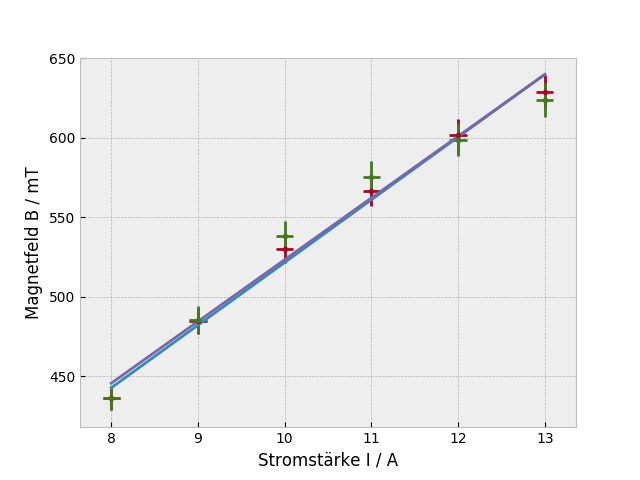
\includegraphics[width=.6\paperwidth]{Auswertung/hysteresis}
      \caption{Hysterese}
      \label{plot::1}
    \end{figure}

  \subsection{Polarisation}
    Das Licht der Cadmium Lampe wird in longitudinaler und transversaler Richtung zum Magnetfeld beobachtet. Durch Verwendung eines linearen Polarisationsfilters und eine $\lambda$/4-Plättchens kann die Polarisation analysiert werden.

    \subsubsection{Beobachtung in longitudinaler Richtung}
      Bei dieser Beobachtungsrichtung sind sowohl mit als auch ohne linearen Polarisationsfilter zwei Linien pro Beugungsordnung zu sehen. Daraus ist zu schließen, dass es sich bei dem Licht um zirkular polarisiertes Licht handelt. (s. \hyperref[pic::1]{Abb. \ref*{pic::1}})

      Wandelt man nun mit Hilfe des $\lambda$/4-Filters das Licht in linear polarisiertes um, so kann man mit dem Polarisationsfilter eine der beiden Linien herausfiltern und bei Rotation um \SI{90}{°} des $\lambda$/4-Filters die jeweils andere beobachten. (s. \hyperref[pic::2]{Abb. \ref*{pic::2}})

      \begin{figure}[H]
        \centering
        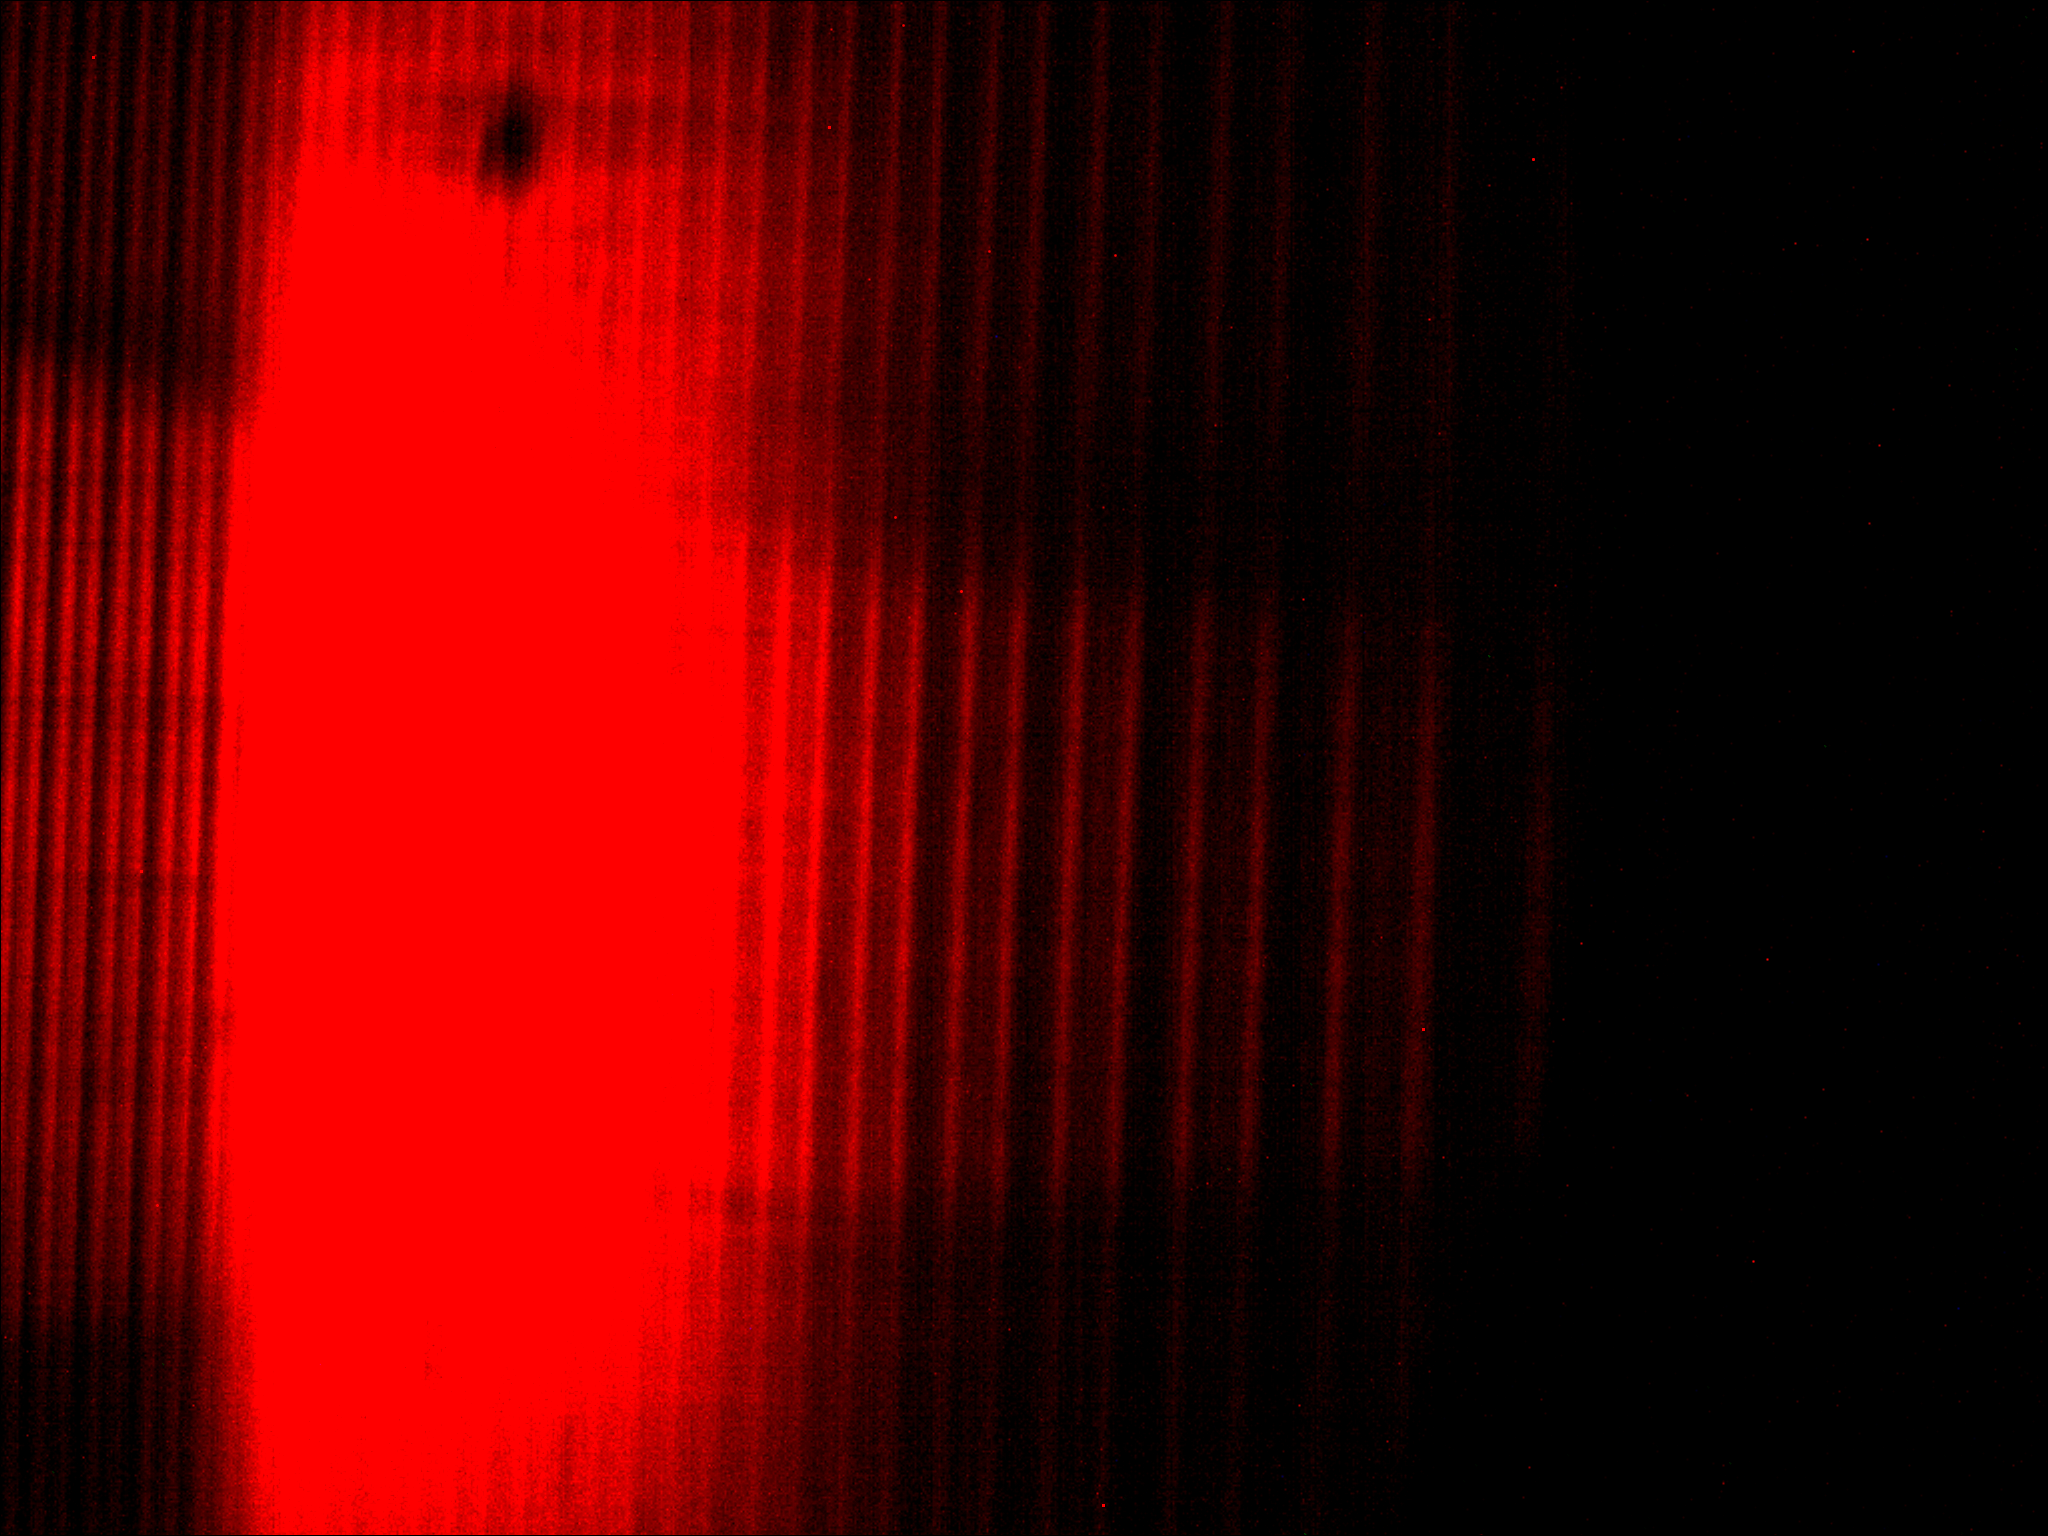
\includegraphics[width=.6\paperwidth, trim={0 200pt 0 400pt}, clip]{Auswertung/data/long/10A_0}
        \caption{Beobachtete Linien in longitudinaler Ausrichtung, ohne Filter}
        \label{pic::1}
      \end{figure}
      \begin{figure}[H]
        \centering
        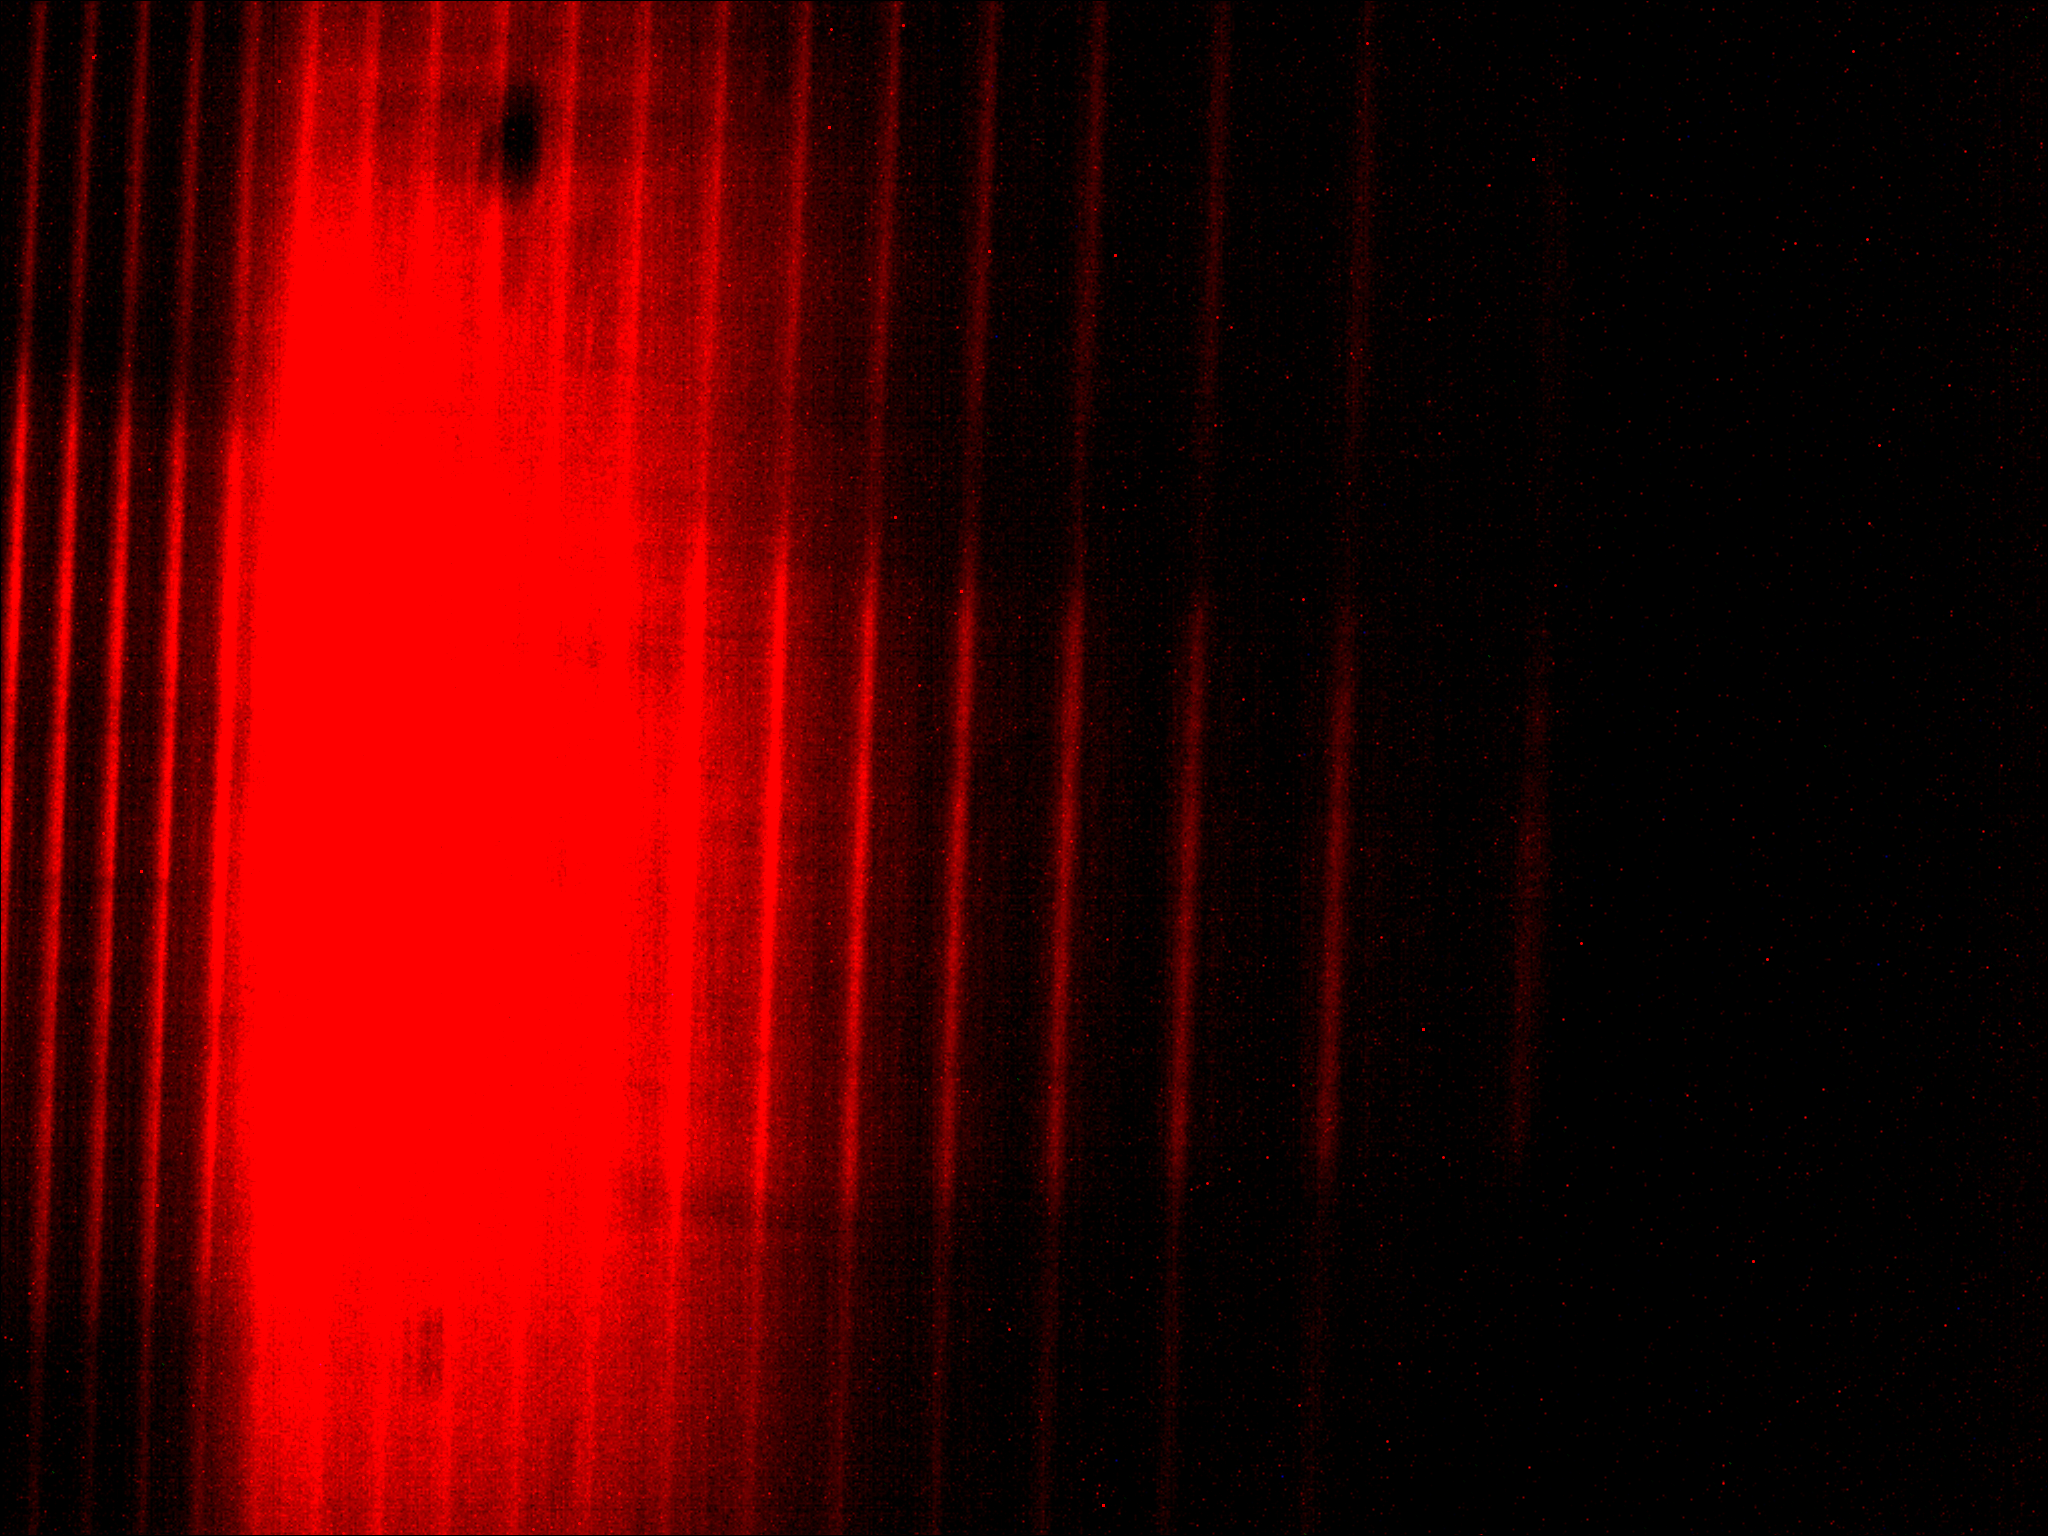
\includegraphics[width=.6\paperwidth, trim={0 650pt 0 200pt}, clip]{Auswertung/data/long/10A_2}
        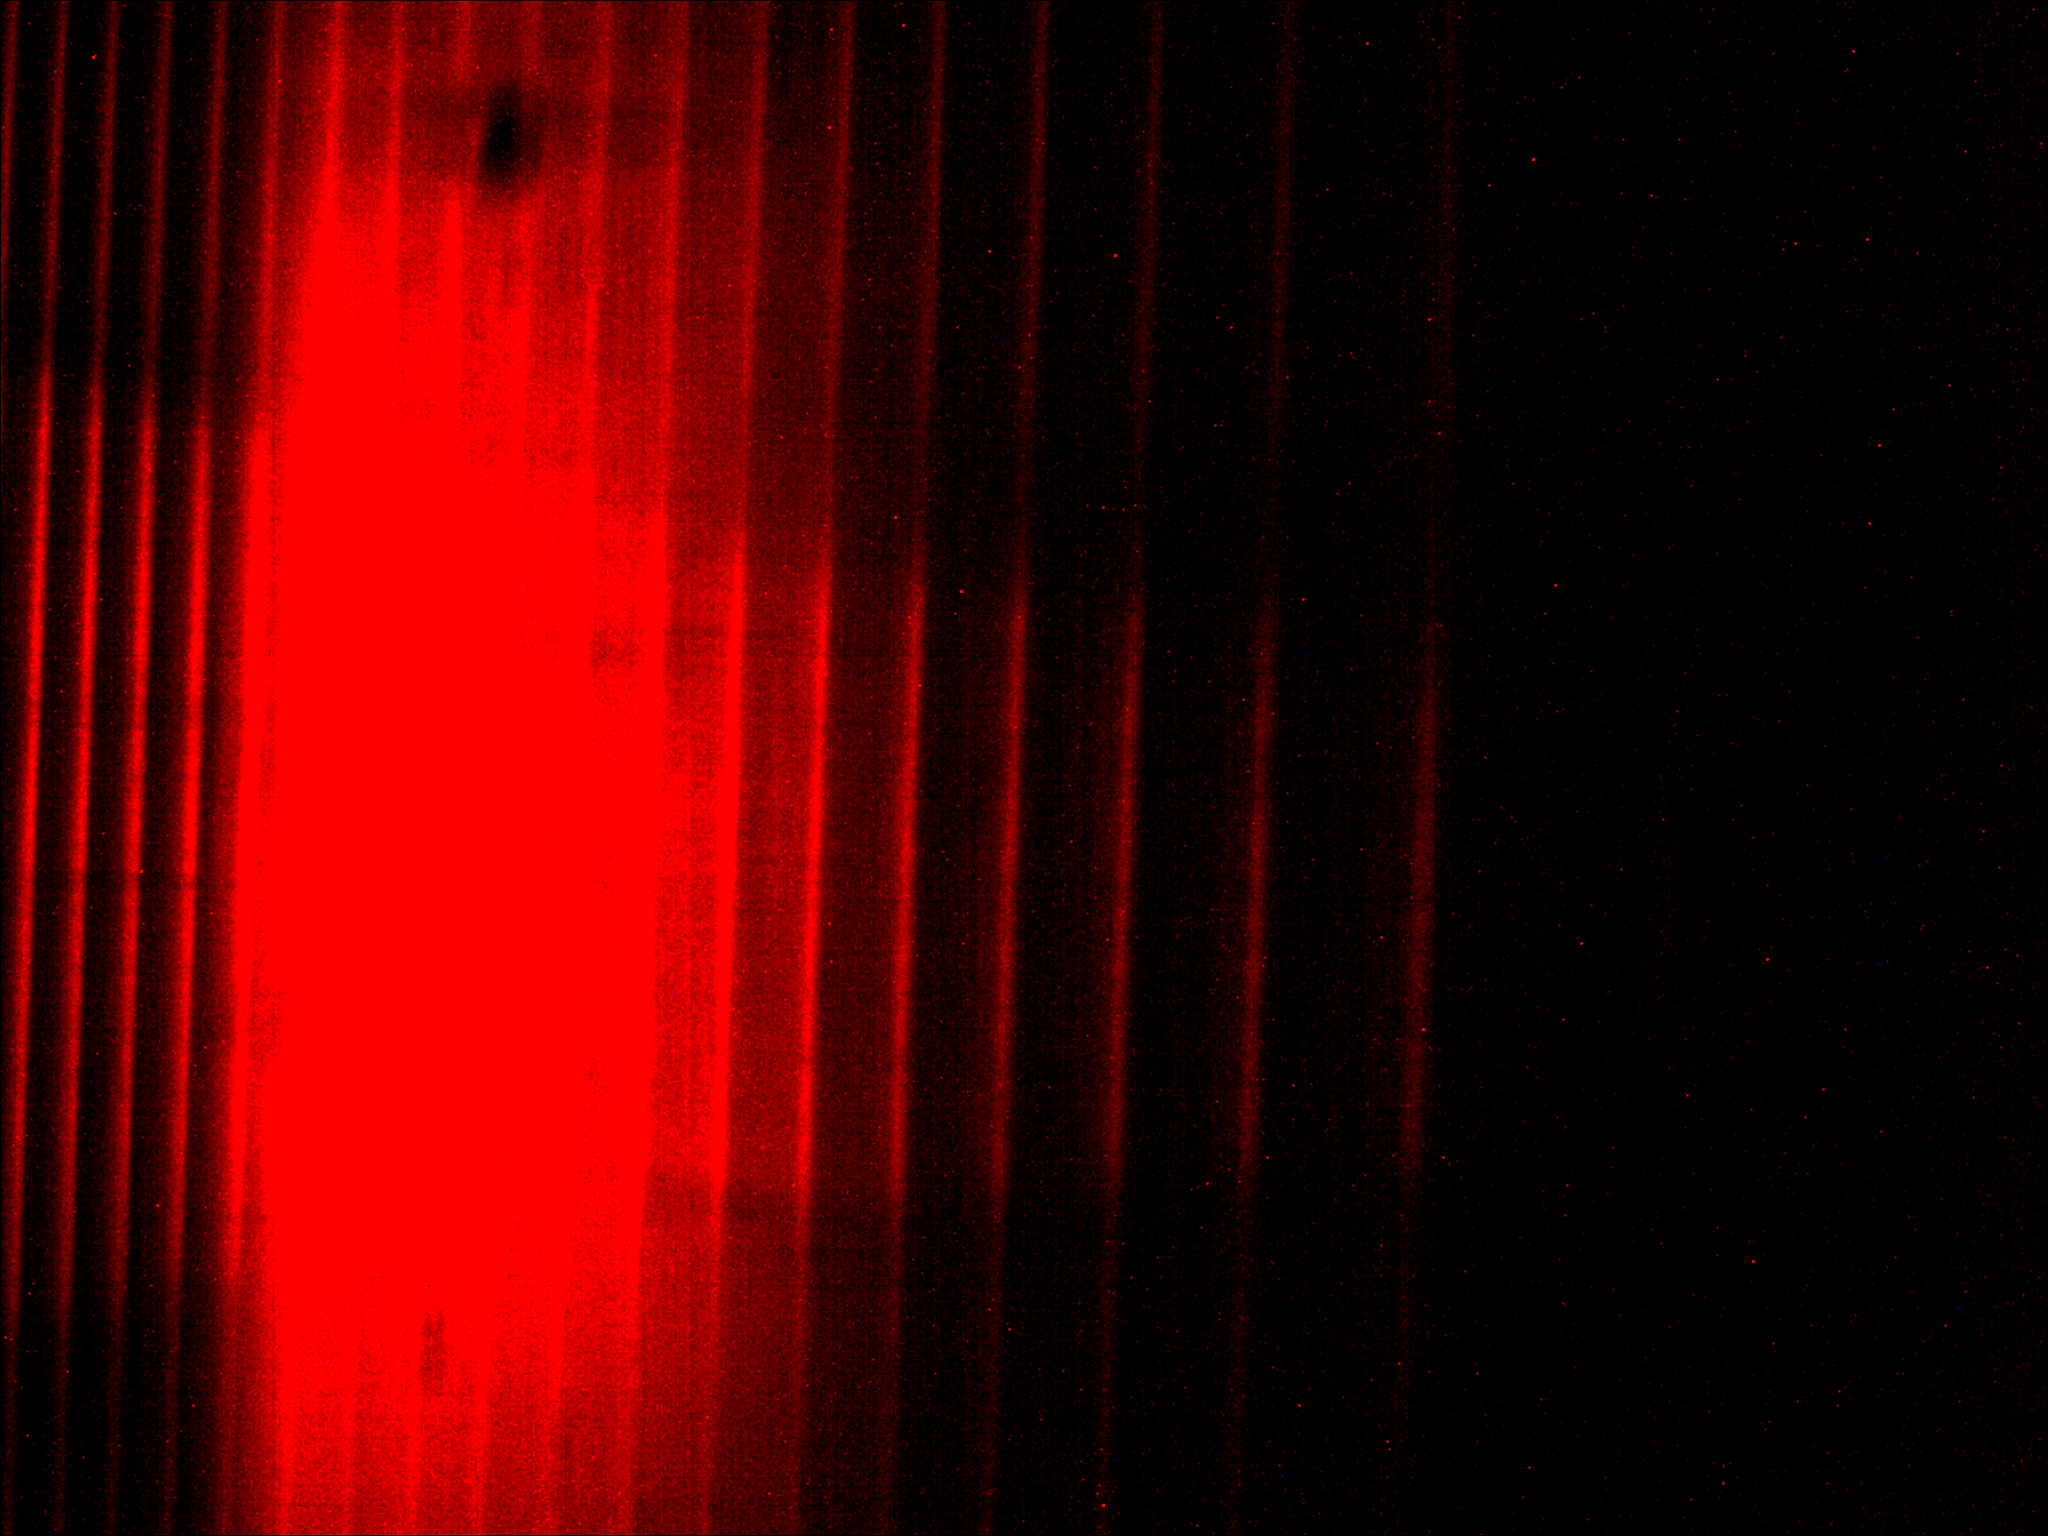
\includegraphics[width=.6\paperwidth, trim={0 0 0 886pt}, clip]{Auswertung/data/long/10A_1}
        \caption{Beobachtete Linien in longitudinaler Richtung, mit $\lambda$/4-Filter und linearem Polarisationsfilter}
        \label{pic::2}
      \end{figure}
    \newpage
    \subsubsection{Beobachtung in transversaler Richtung}
      Hier können wir eine Aufspaltung in drei Linien beobachten. Der Polarisationsfilter lässt entweder die beiden äusseren Linen ($\sigma$-Linien) verschwinden, oder nach einer \SI{90}{°} Drehung die mittlere Linie ($\pi$-Linie) (s. \hyperref[pic::3]{Abb. \ref*{pic::3}}). Das Licht ist also linear polarisiert, mit senkrechter Polarisationsrichtung zwichen $\sigma$- und $\pi$-Linien

      \begin{figure}[H]
        \centering
        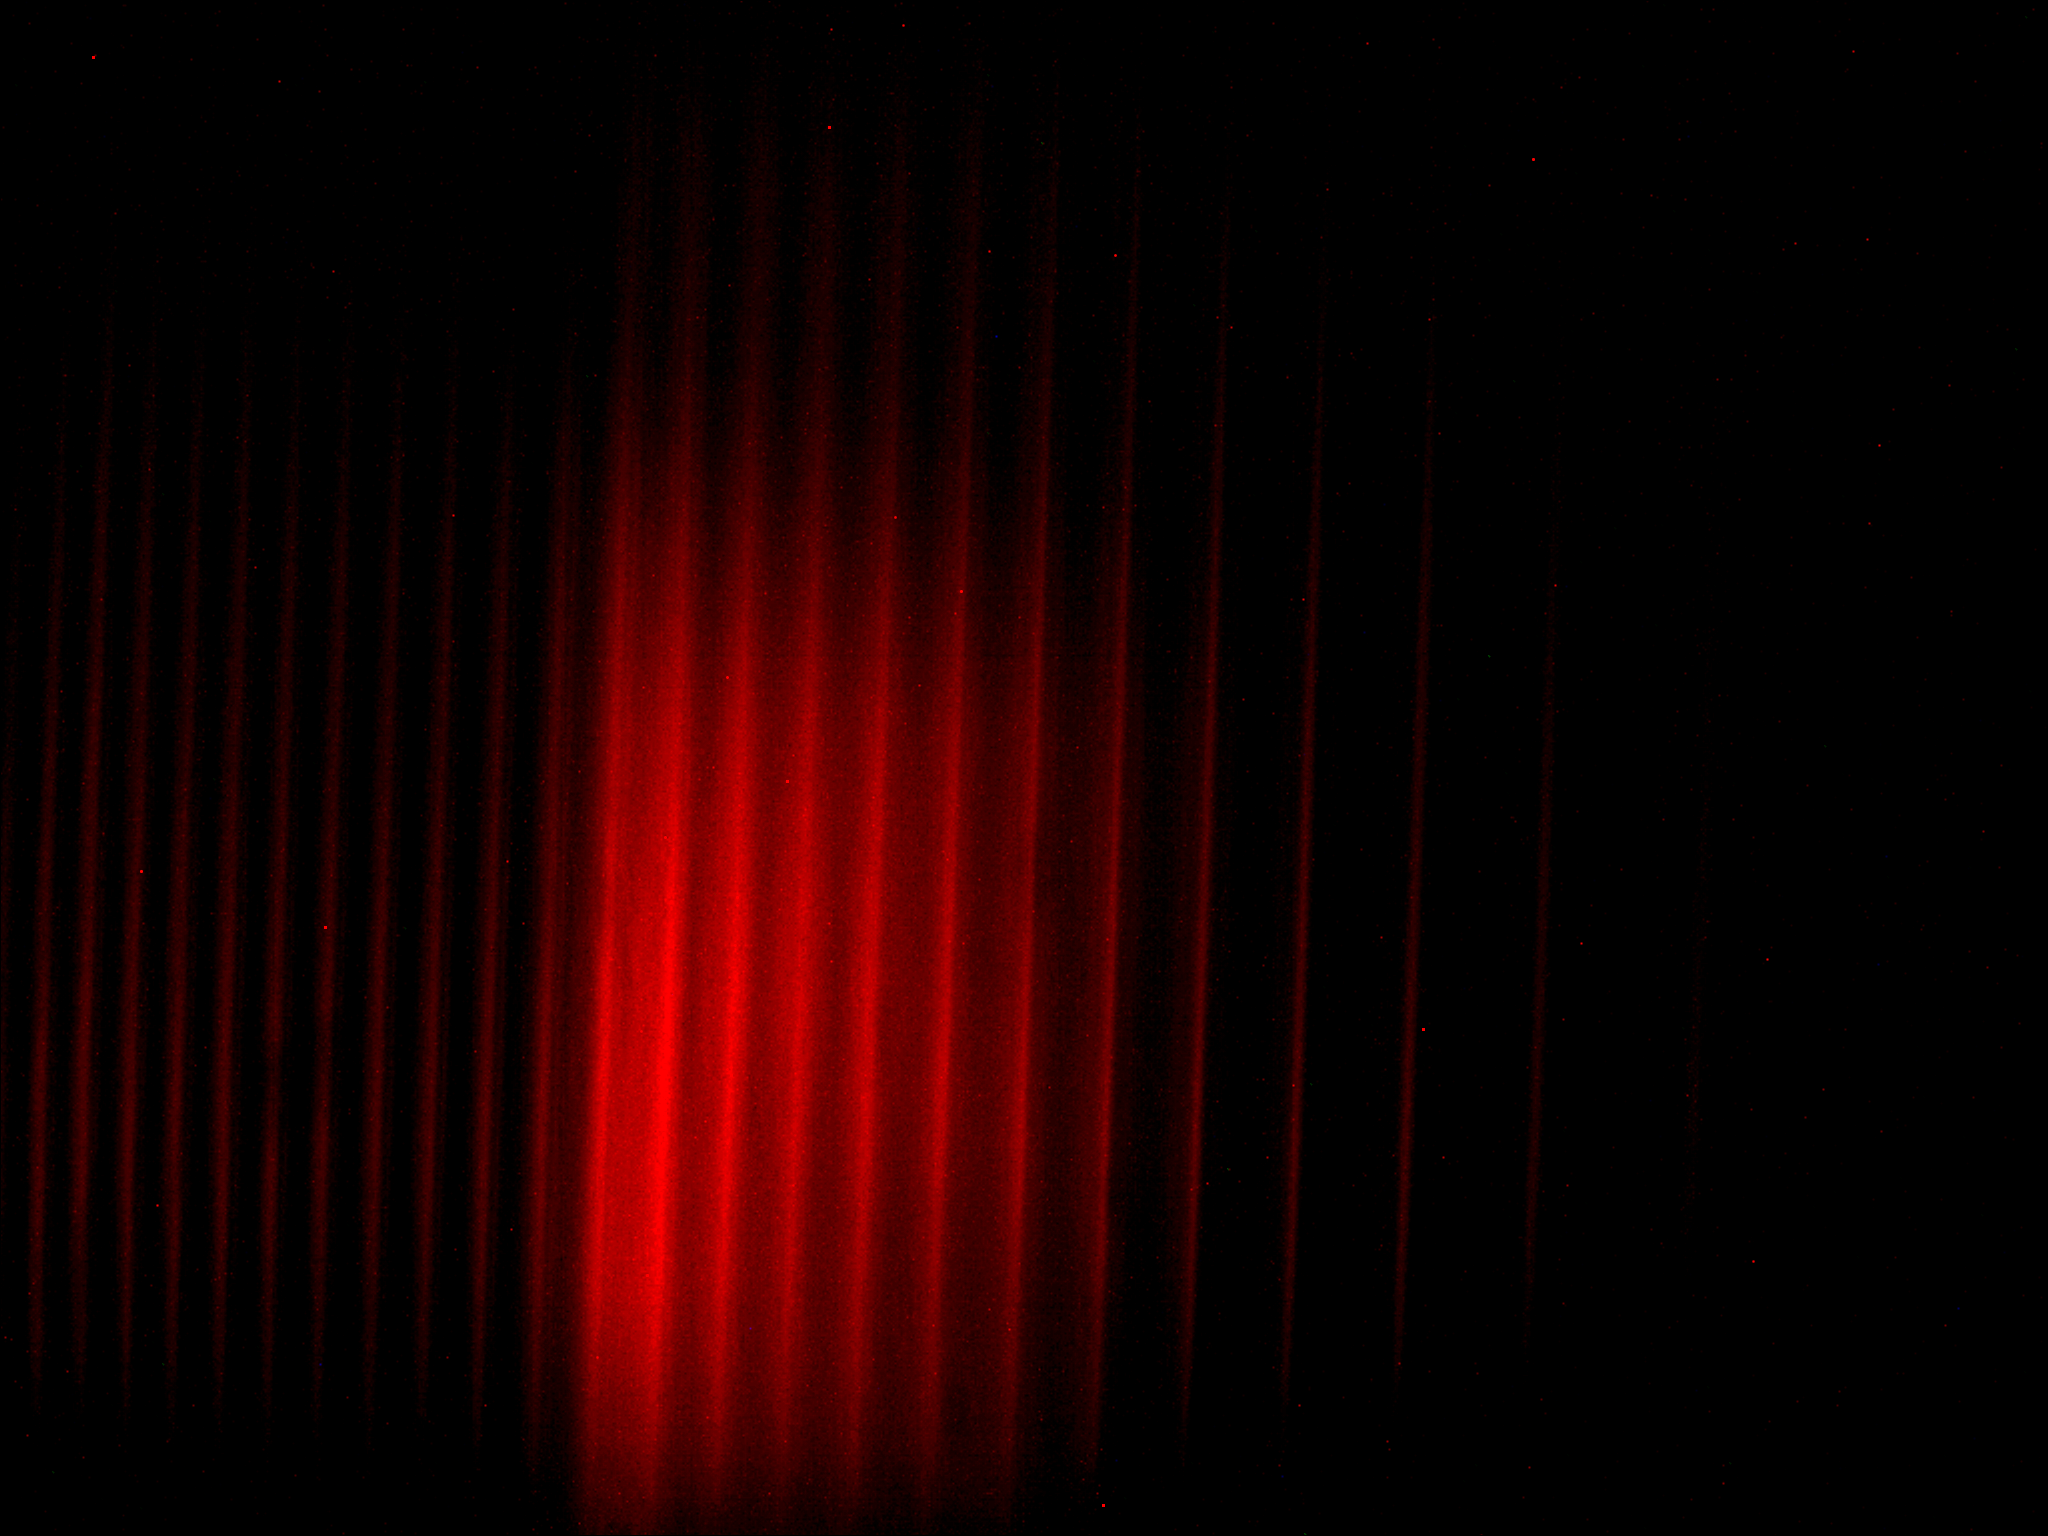
\includegraphics[width=.6\paperwidth, trim={0 300pt 0 900pt}, clip]{Auswertung/data/trans/10A/10A_pi}
        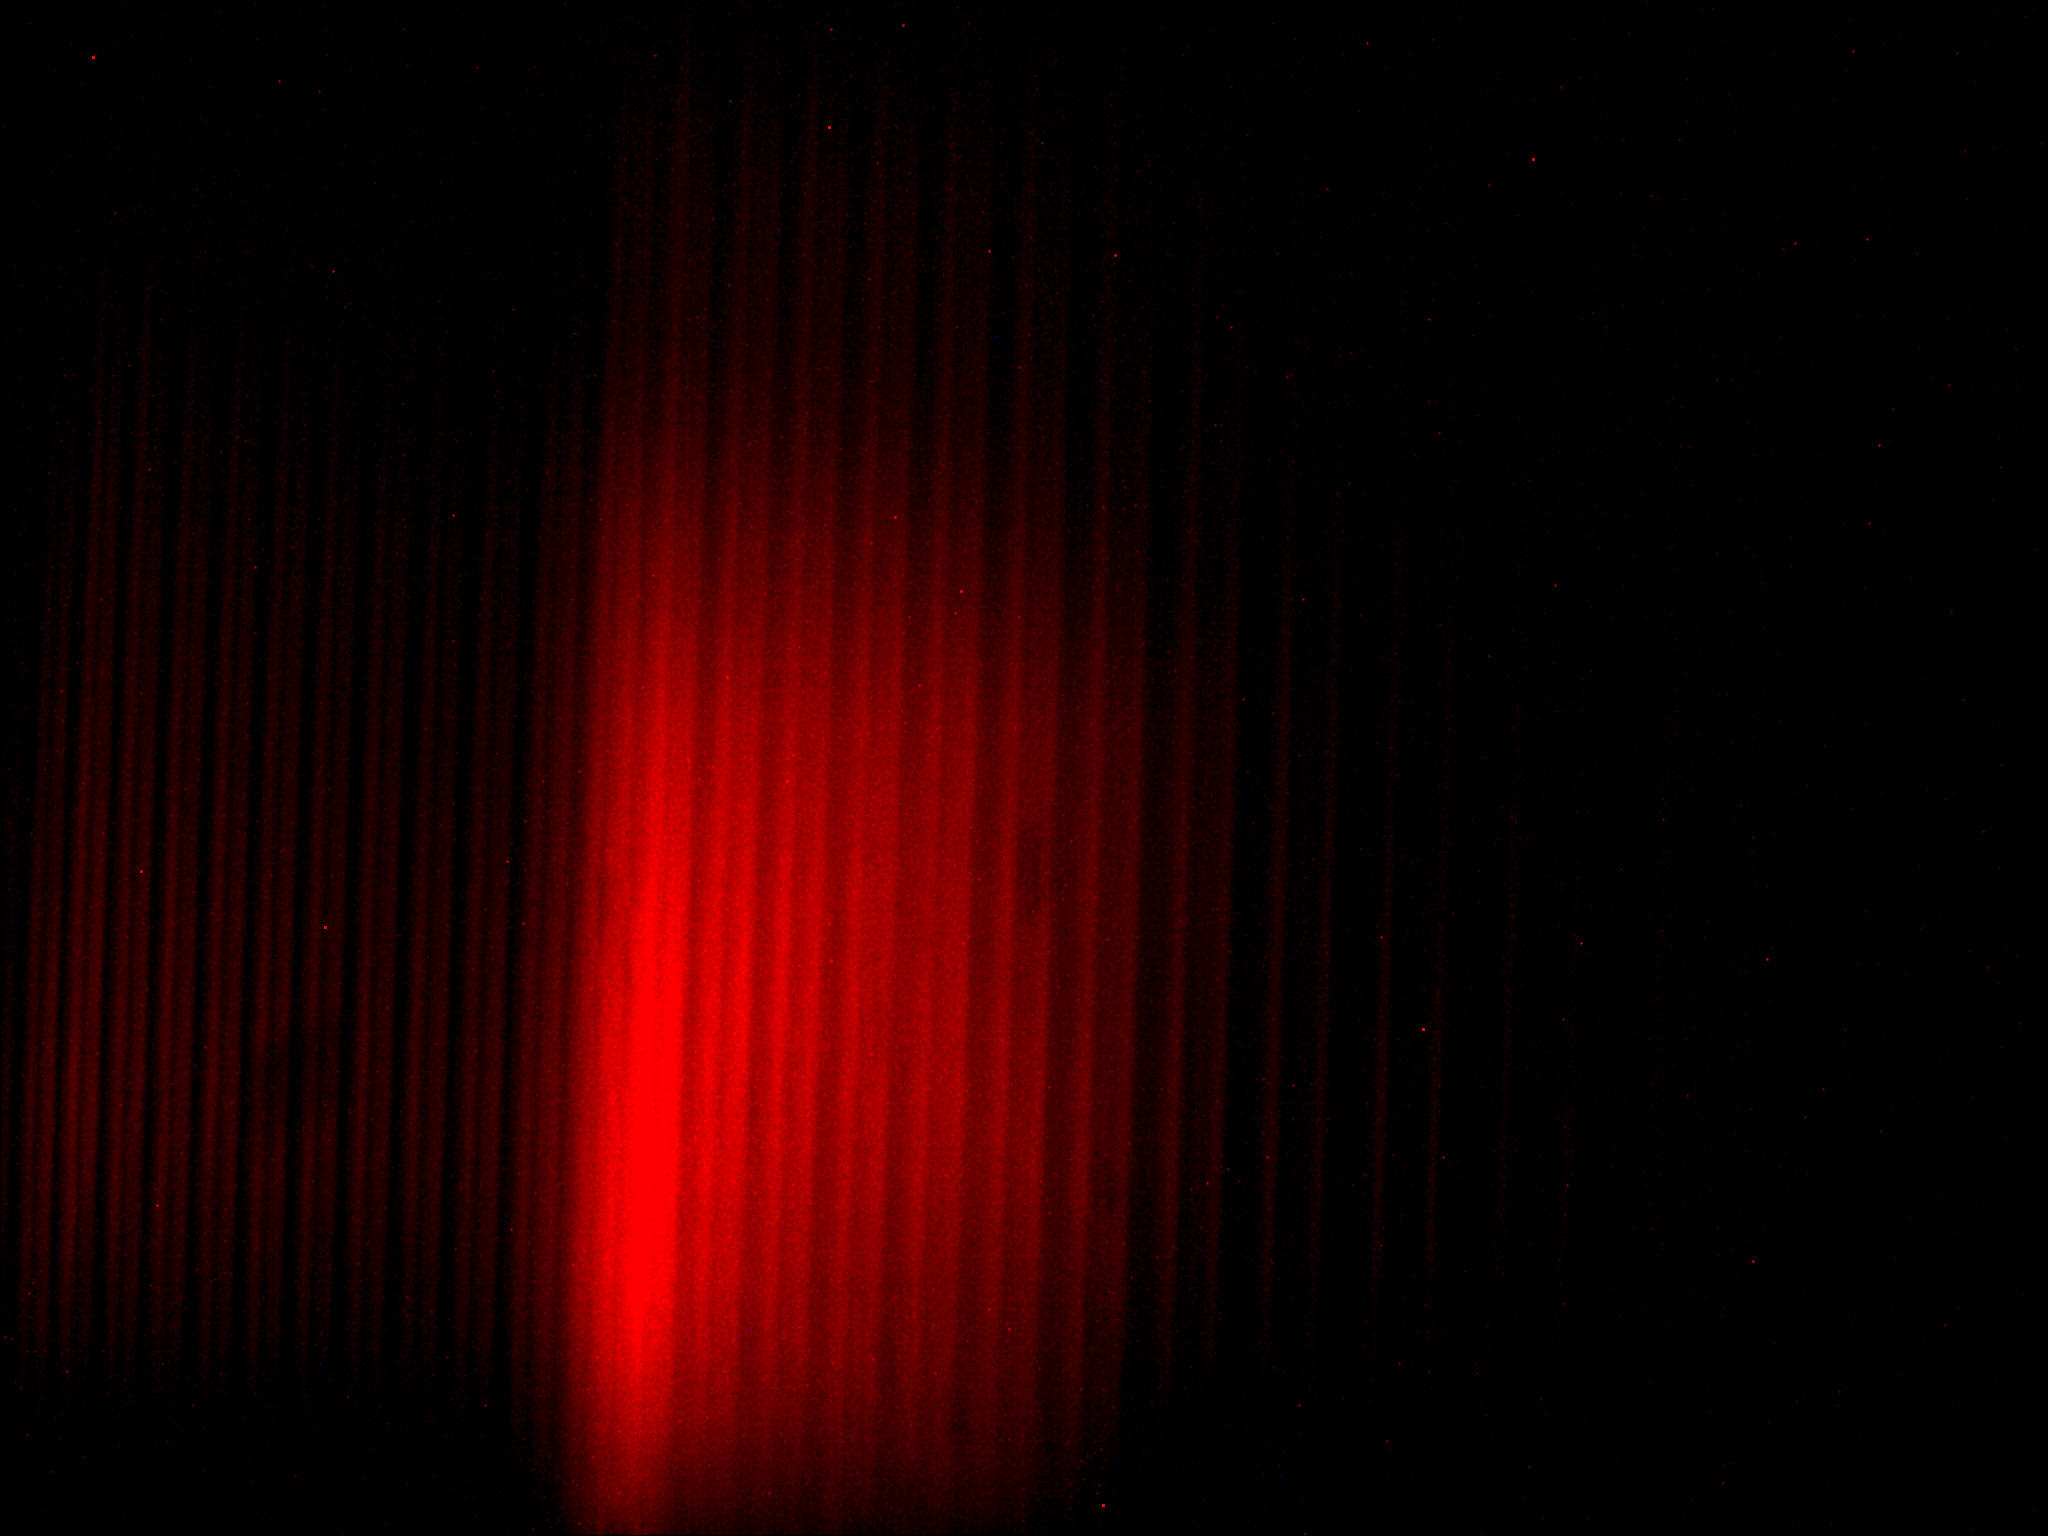
\includegraphics[width=.6\paperwidth, trim={0 300pt 0 900pt}, clip]{Auswertung/data/trans/10A/10A_sig}
        \caption{Beobachtete Linien in transversaler Ausrichtung, mit linearem Polarisationsfilter}
        \label{pic::3}
      \end{figure}

      Bei Variation der Stromstärke und des damit resultierenden Magnetfeldes, kann man beobachten, dass die Aufspaltung der Spektrallinien mit zunehmender Stromstärke größer wird.

      \begin{figure}[H]
        \centering
        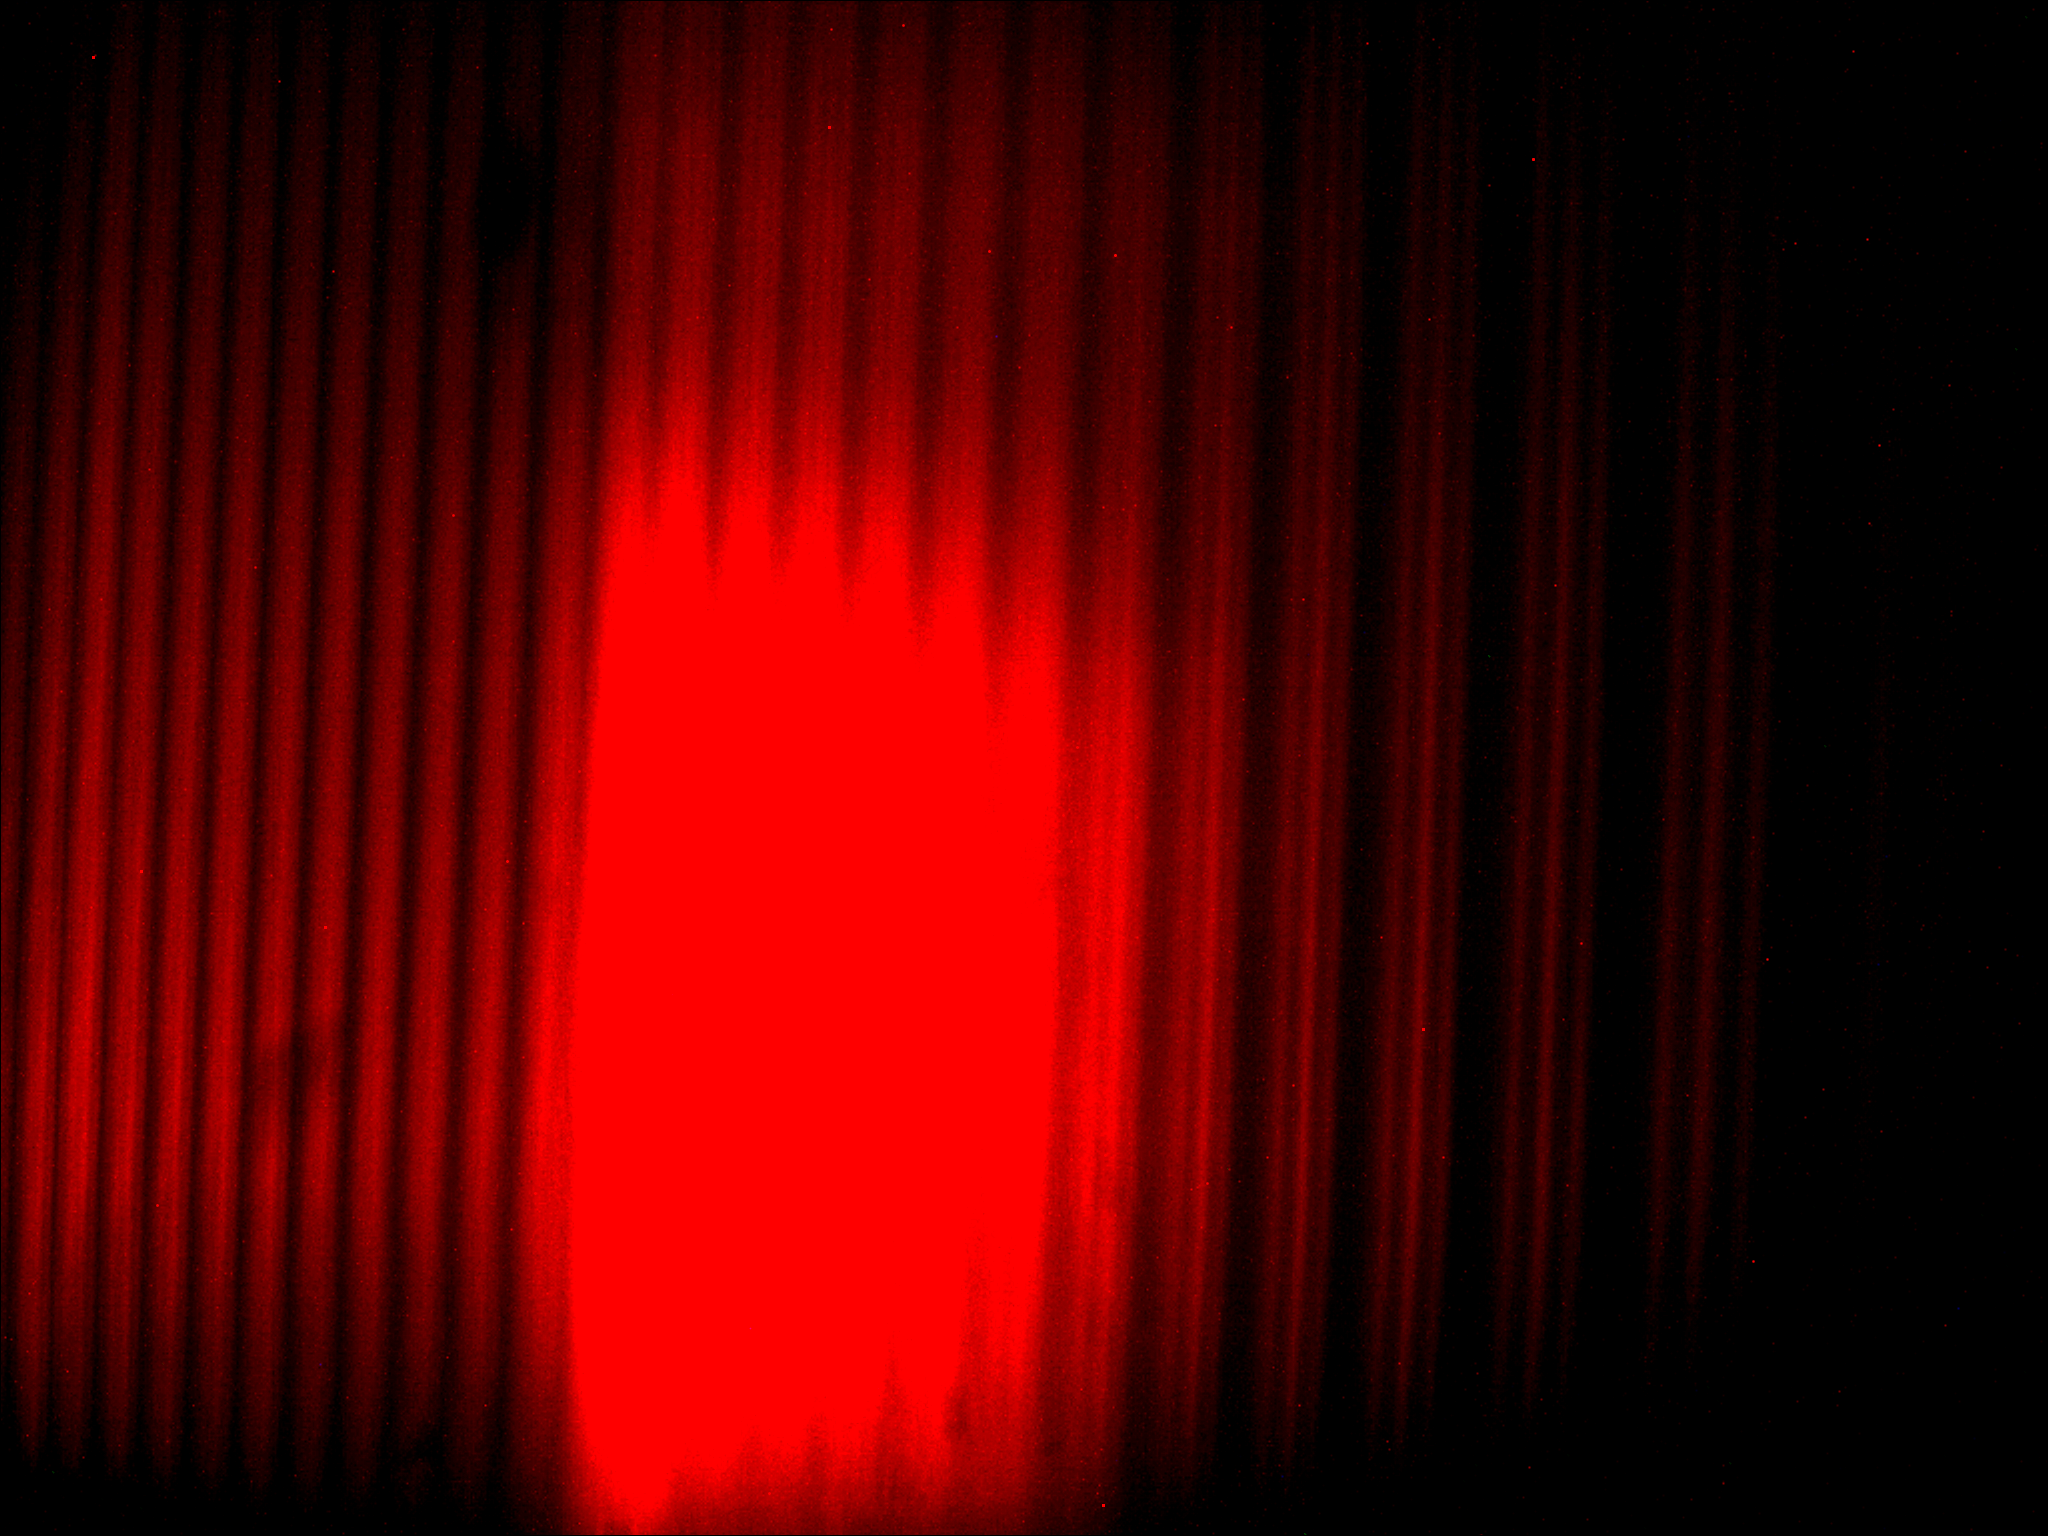
\includegraphics[width=.6\paperwidth,trim={0 600pt 0 500pt}, clip]{Auswertung/data/trans/10A/10A_l}
        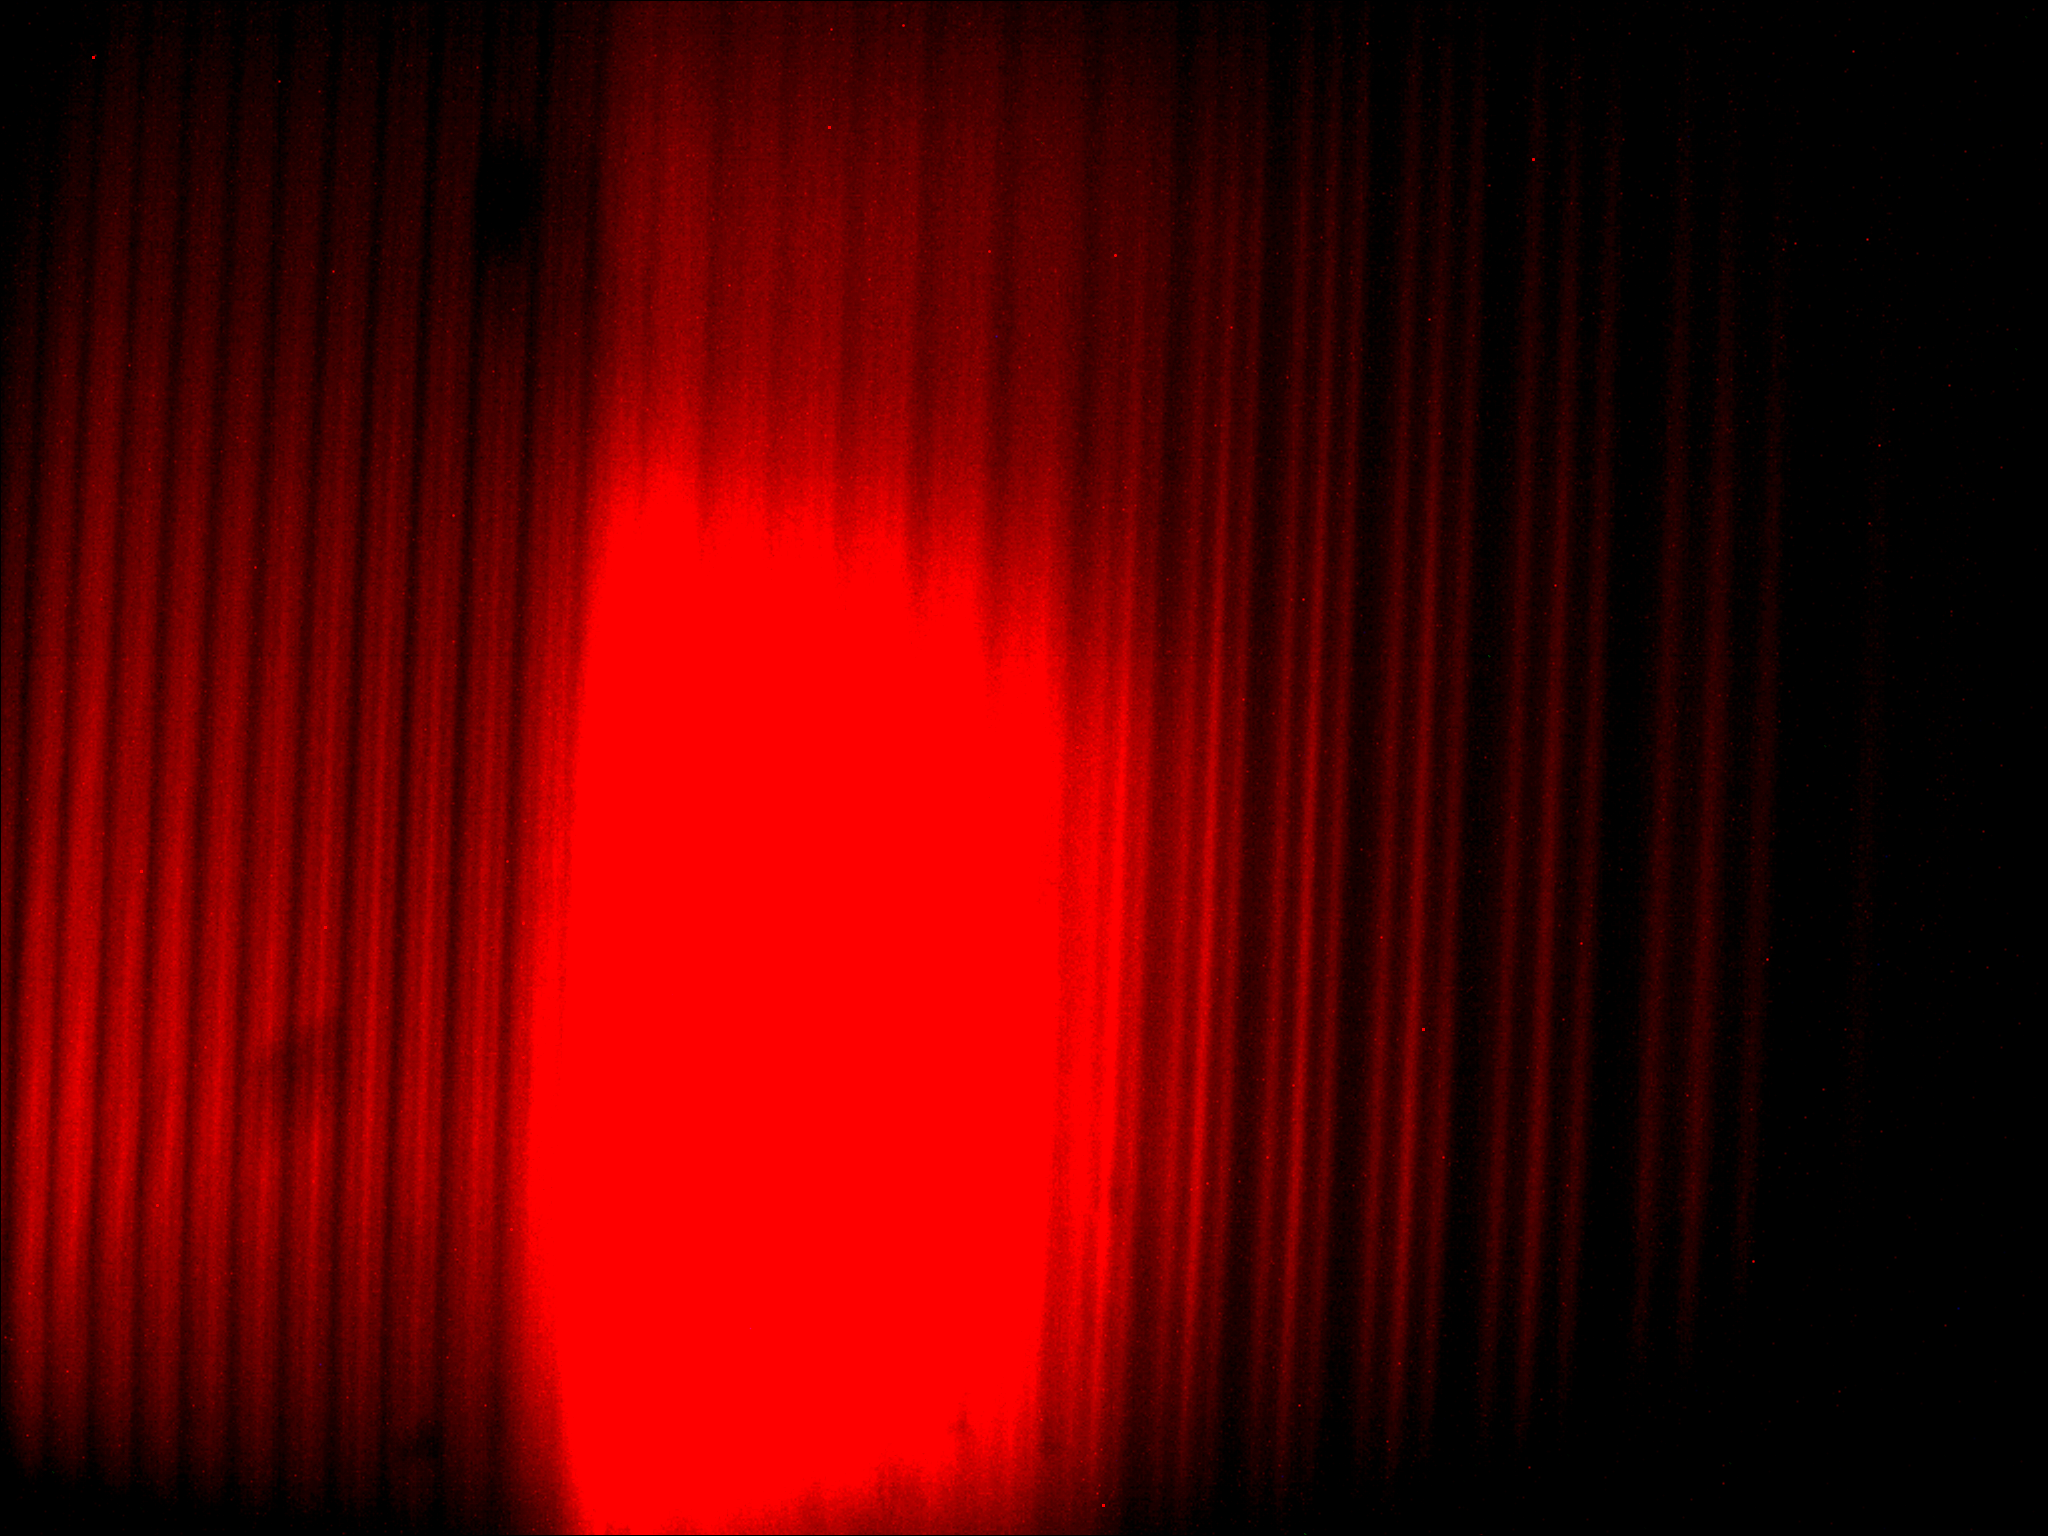
\includegraphics[width=.6\paperwidth,trim={0 200pt 0 900pt}, clip]{Auswertung/data/trans/13A/13A_l}
        \caption{Beobachtete Linien in transversaler Richtung, bei 10A (oben) und 13A (unten)}
        \label{pic::4}
      \end{figure}

    \subsection{Bestimmung der Wellenlängenverschiebung}
      \subsubsection{Position der $\pi$- und $\sigma$-Linien}
        Wir nutzen das Programm \textbf{JImage} um die zweidimensionalen Bilder, der beobachteten spektralen Aufspaltung in eine eindimensionale Intensitätsverteilung zu konvertieren. Mit \textbf{Python}\footnote{Repo mit den benutzten Skripten zur Auswertung:  \href{github.com/acereca/FP/tree/master/F44 - Zeemanspektroskopie}{github.com/acereca/FP $\rightarrow$ F44}} kann jetzt die Position (in Pixel) jeder $\pi$- und $\sigma$-Linie von etwa fünf Ordnungen (wegen der Reflektion in der Mitte der Bilder) pro Messung bestimmt werden.

        Jeder gemessene Peak wird jetzt mit einer Gausskurve gefittet und daraus die Breite und Position bestimmt. Die Gaussfunktion berücksichtigt, dass durch die thermische Bewegung der Atome ein Doppler-Effekt entsteht und dadurch ist die ausgesandte Wellenlänge je nach Bewegungsrichtung des Atoms leicht verschoben, sodass die Linien im Vergleich zur Lorentz-Kurve breiter erscheinen. Als Fehler der Position wird hier der $\sigma^2$-Parameter der Gaussfunktion genutzt
        \begin{align}
          \Delta x = \sigma \cdot 2.4 / 2
        \end{align}
        also die halbe Halbwertsbreite (HWHM).

      \subsubsection{Verschiebung der Ordungen}
        Wir ordnen nun den $\pi$-Linien Ordnungszahlen zu, diese sollten nur diskrete, ganzzahlige Werte sein, allerdings möchten wir den $\sigma$-Linien auch eine solche Ordnung zuordnen, also betrachten wir eine kontinuierliche Fitfunktion. In unserem Fall ist diese eine Polynomfunktion 2. Grades (s. \hyperref[plot::2]{Abb. \ref*{plot::2}}). Diese Beobachtung ist innerhalb unserer Näherung ausreichend, da ein Polynom höheren Grades keine signifikante Verbesserung der Beschreibung unserer Daten liefert.

        Um die Fehler der Beugungsordnung zu bestimmen nutzen wir:
        \begin{align}
          \Delta k(a) = k(a+\Delta a) - k(a)
        \end{align}
        wobei die Fehler der Fitparameter vernachlässigt werden. $a$ ist hier die Position der Linien in Pixel, $k$ die zugeordnete Beugungsordnung.

        Jetzt werden die Verschiebungen der $\sigma$-Linien zur zugehörigen $\pi$-Linie, in Bruchteilen einer Beugungsordnung, berechnet und geplottet (\hyperref[plot::3]{Abb. \ref*{plot::3}}), für die Berechnung dient:
        \begin{align}
          \delta k = k(a) - k_{theo}\\
          \Delta (\delta k) = \Delta k(a)
        \end{align}
        Dabei entspricht die theoretische Beugungsordnung $k_{theo}$ den diskreten Werten, die den $\pi$-Linien zugeornet werden können. Der Fehler geht hier aus dem Fehler der errechneten Beugungsordung der $\sigma$-Linien hervor, da $k_{theo}$ keinen Fehler besitzt.

        \begin{landscape}
          \thispagestyle{empty}
          \begin{figure}
            \vspace*{-2cm}
            \caption{Gefittete Positionen der Peaks}
            \label{plot::2}
            \hspace*{-6cm}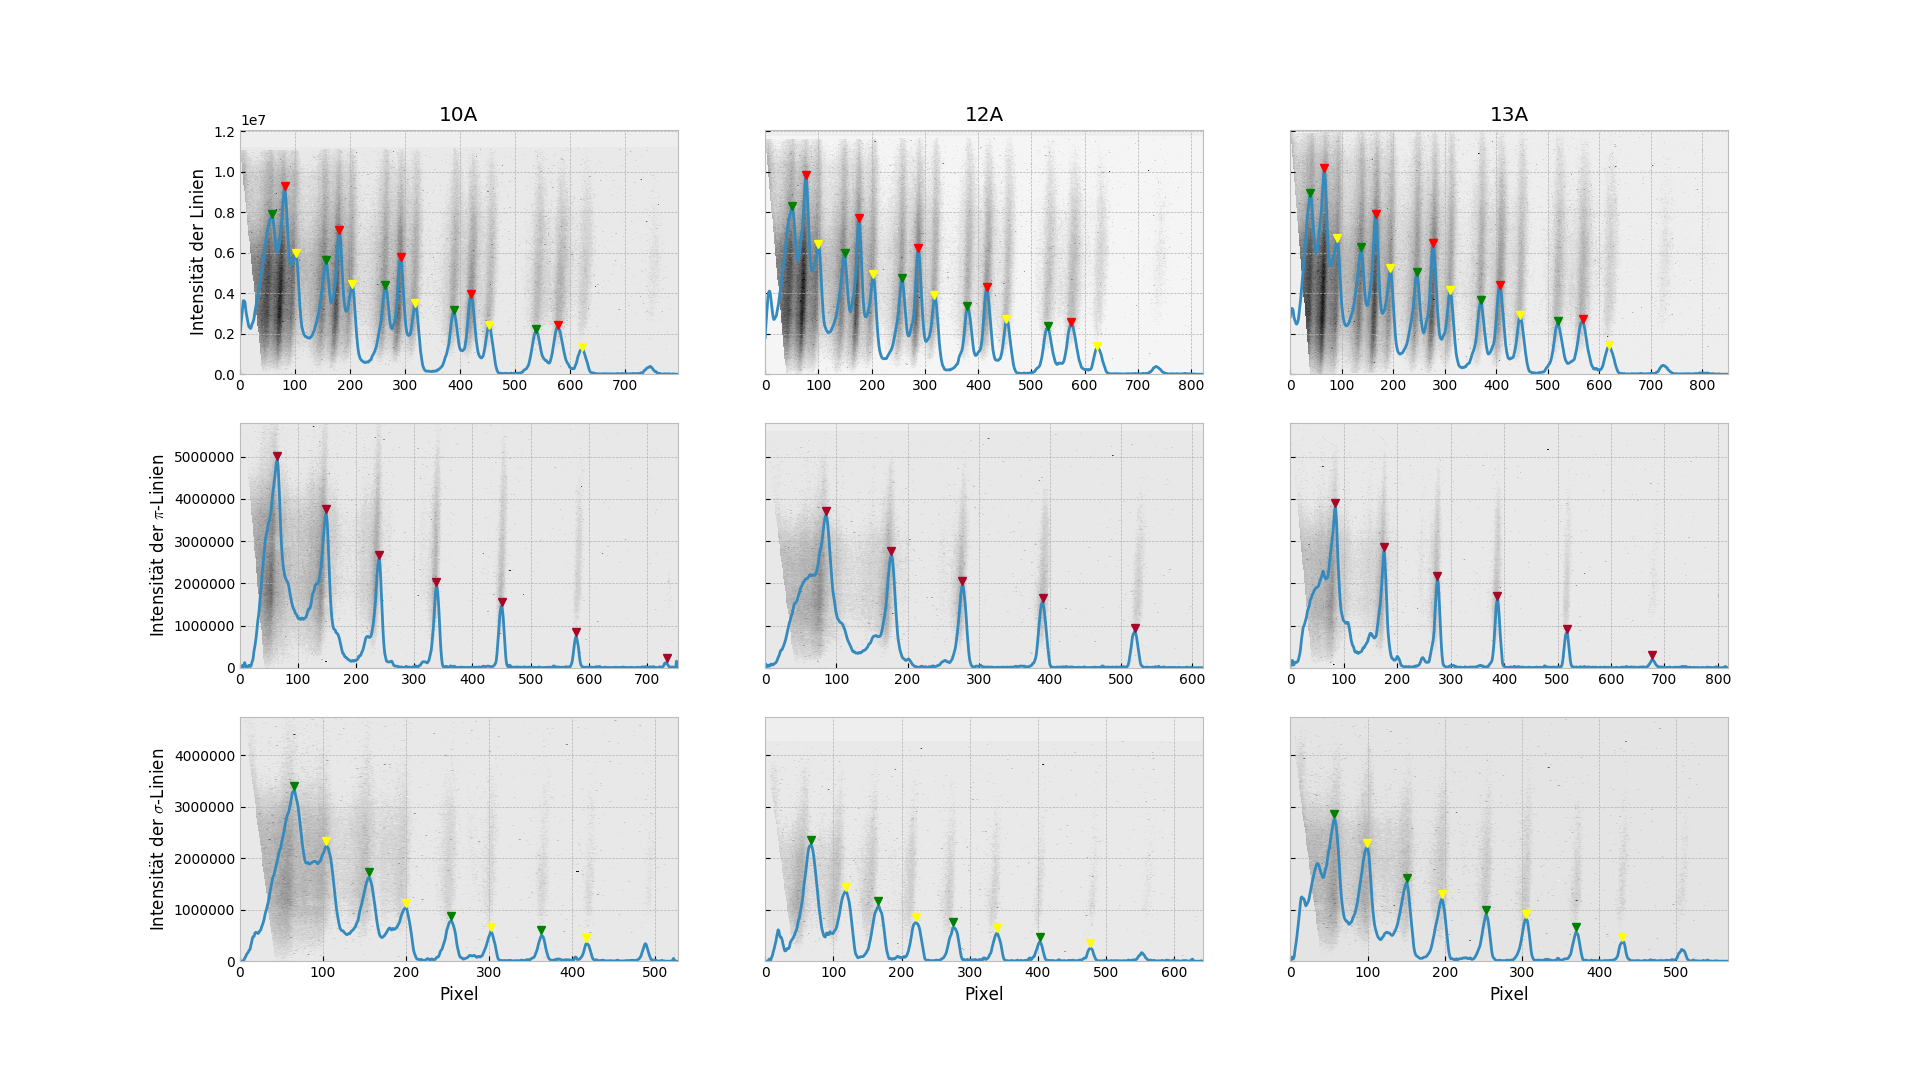
\includegraphics[width=1.5\paperwidth]{Auswertung/peaks}
          \end{figure}
        \end{landscape}
        \begin{landscape}
          \thispagestyle{empty}
          \begin{figure}
            \vspace*{-2cm}
            \caption{Polynomfits für die drei Stromstärken}
            \label{plot::3}
            \hspace*{-5cm}
            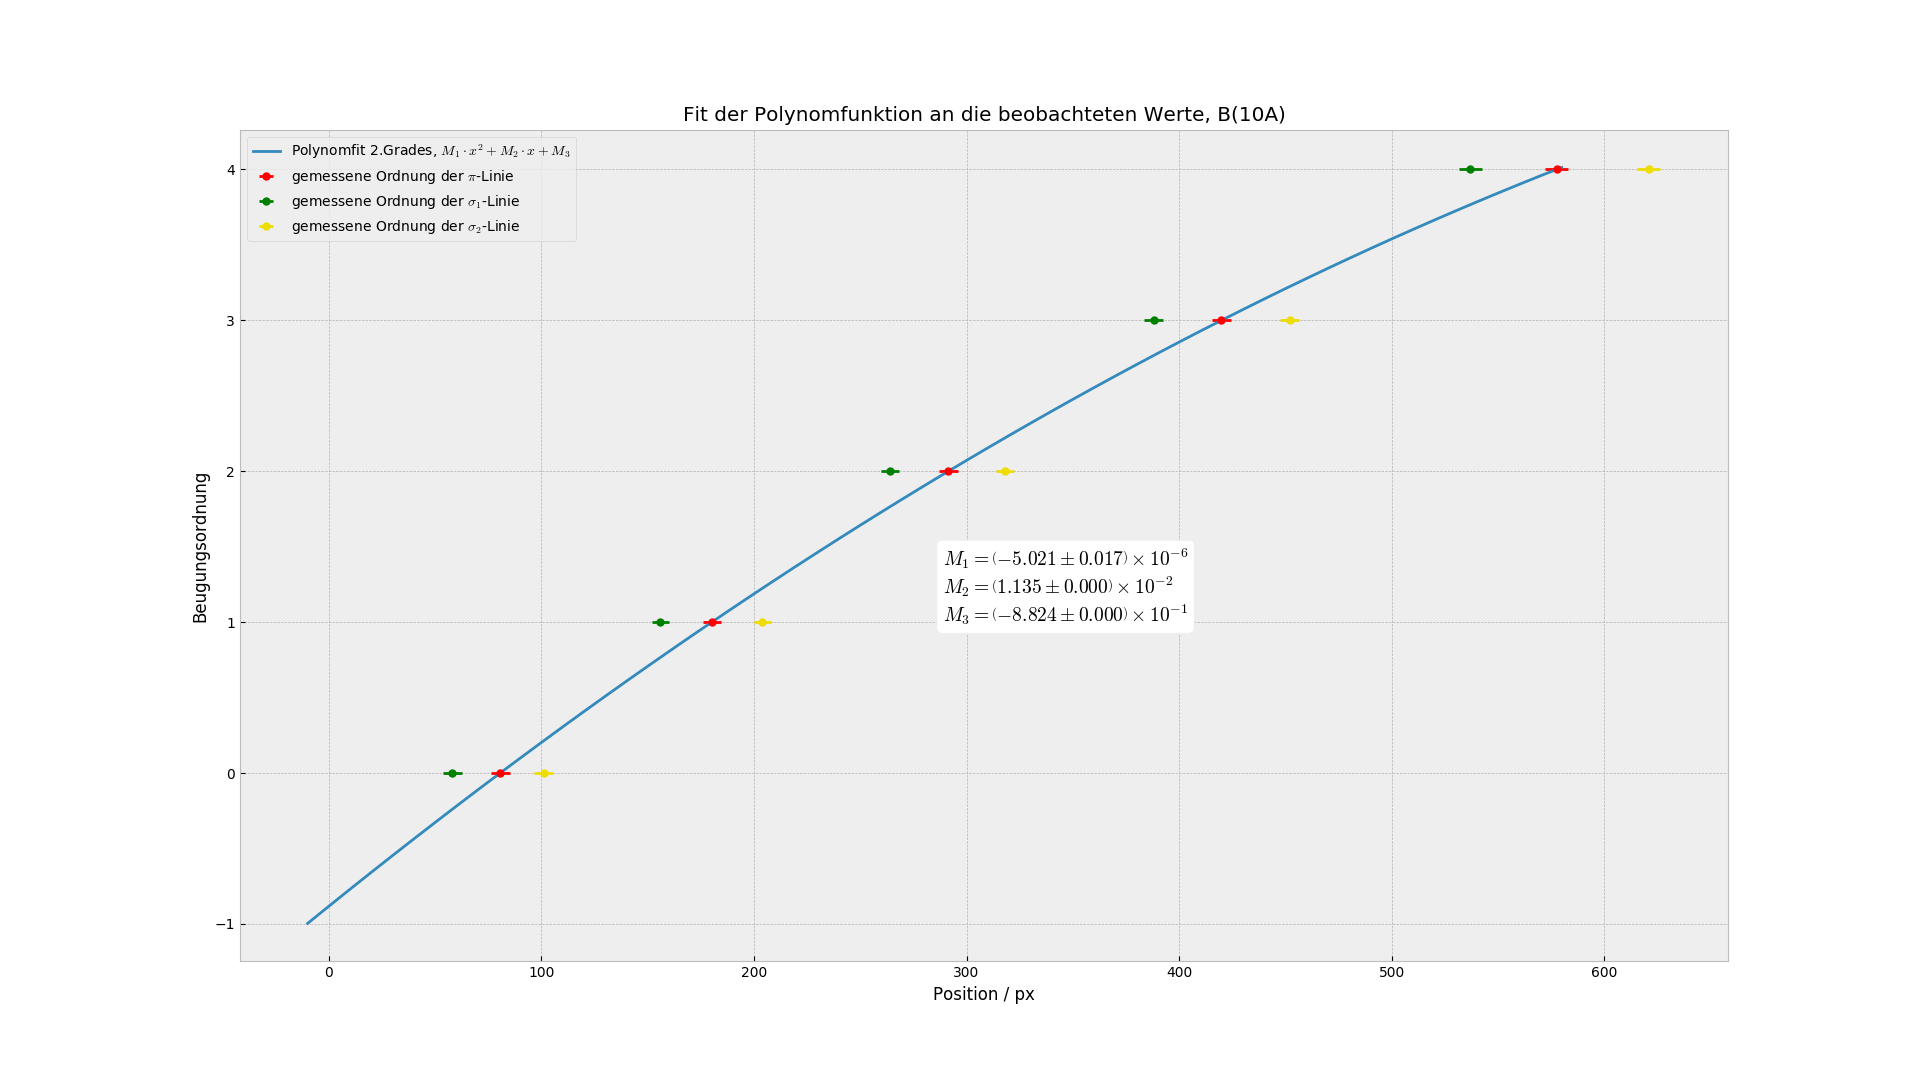
\includegraphics[width=.45\paperwidth]{Auswertung/scatterorder/sco_10A}
            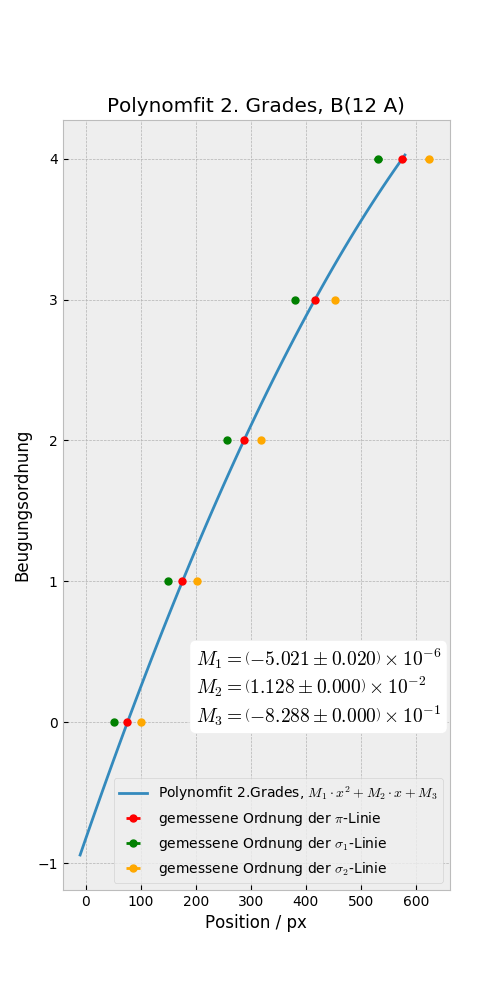
\includegraphics[width=.45\paperwidth]{Auswertung/scatterorder/sco_12A}
            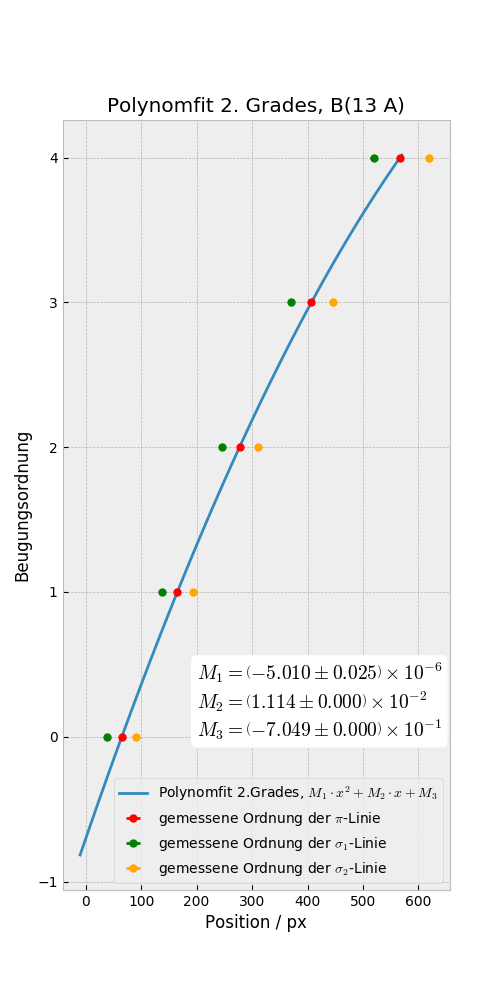
\includegraphics[width=.45\paperwidth]{Auswertung/scatterorder/sco_13A}
          \end{figure}
        \end{landscape}
        \begin{landscape}
          \thispagestyle{empty}
          \begin{figure}
            \vspace*{-2cm}
            \caption{Verschiebung der Beugungsordnung}
            \label{plot::3.5}
            \hspace*{-5cm}\vspace{-1cm}
            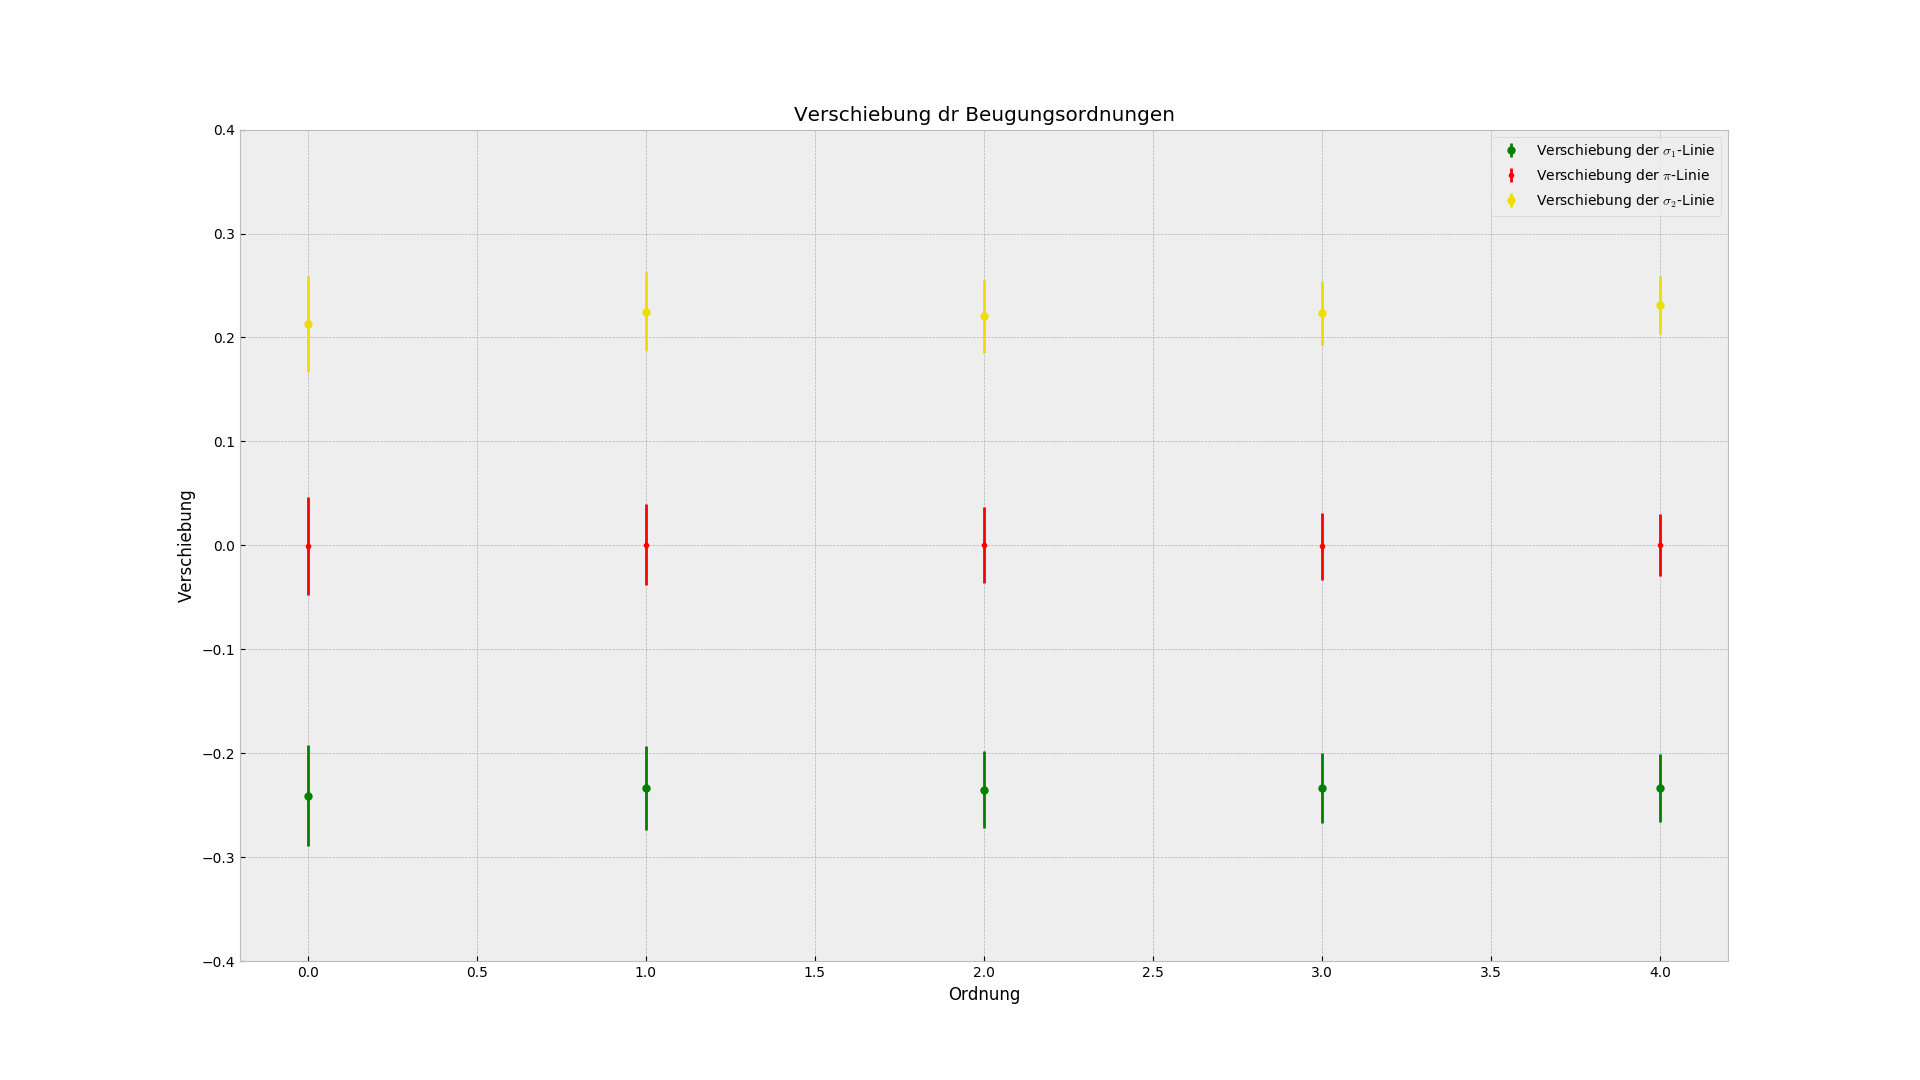
\includegraphics[width=.45\paperwidth]{Auswertung/scatterorder/diff_sco10A}
            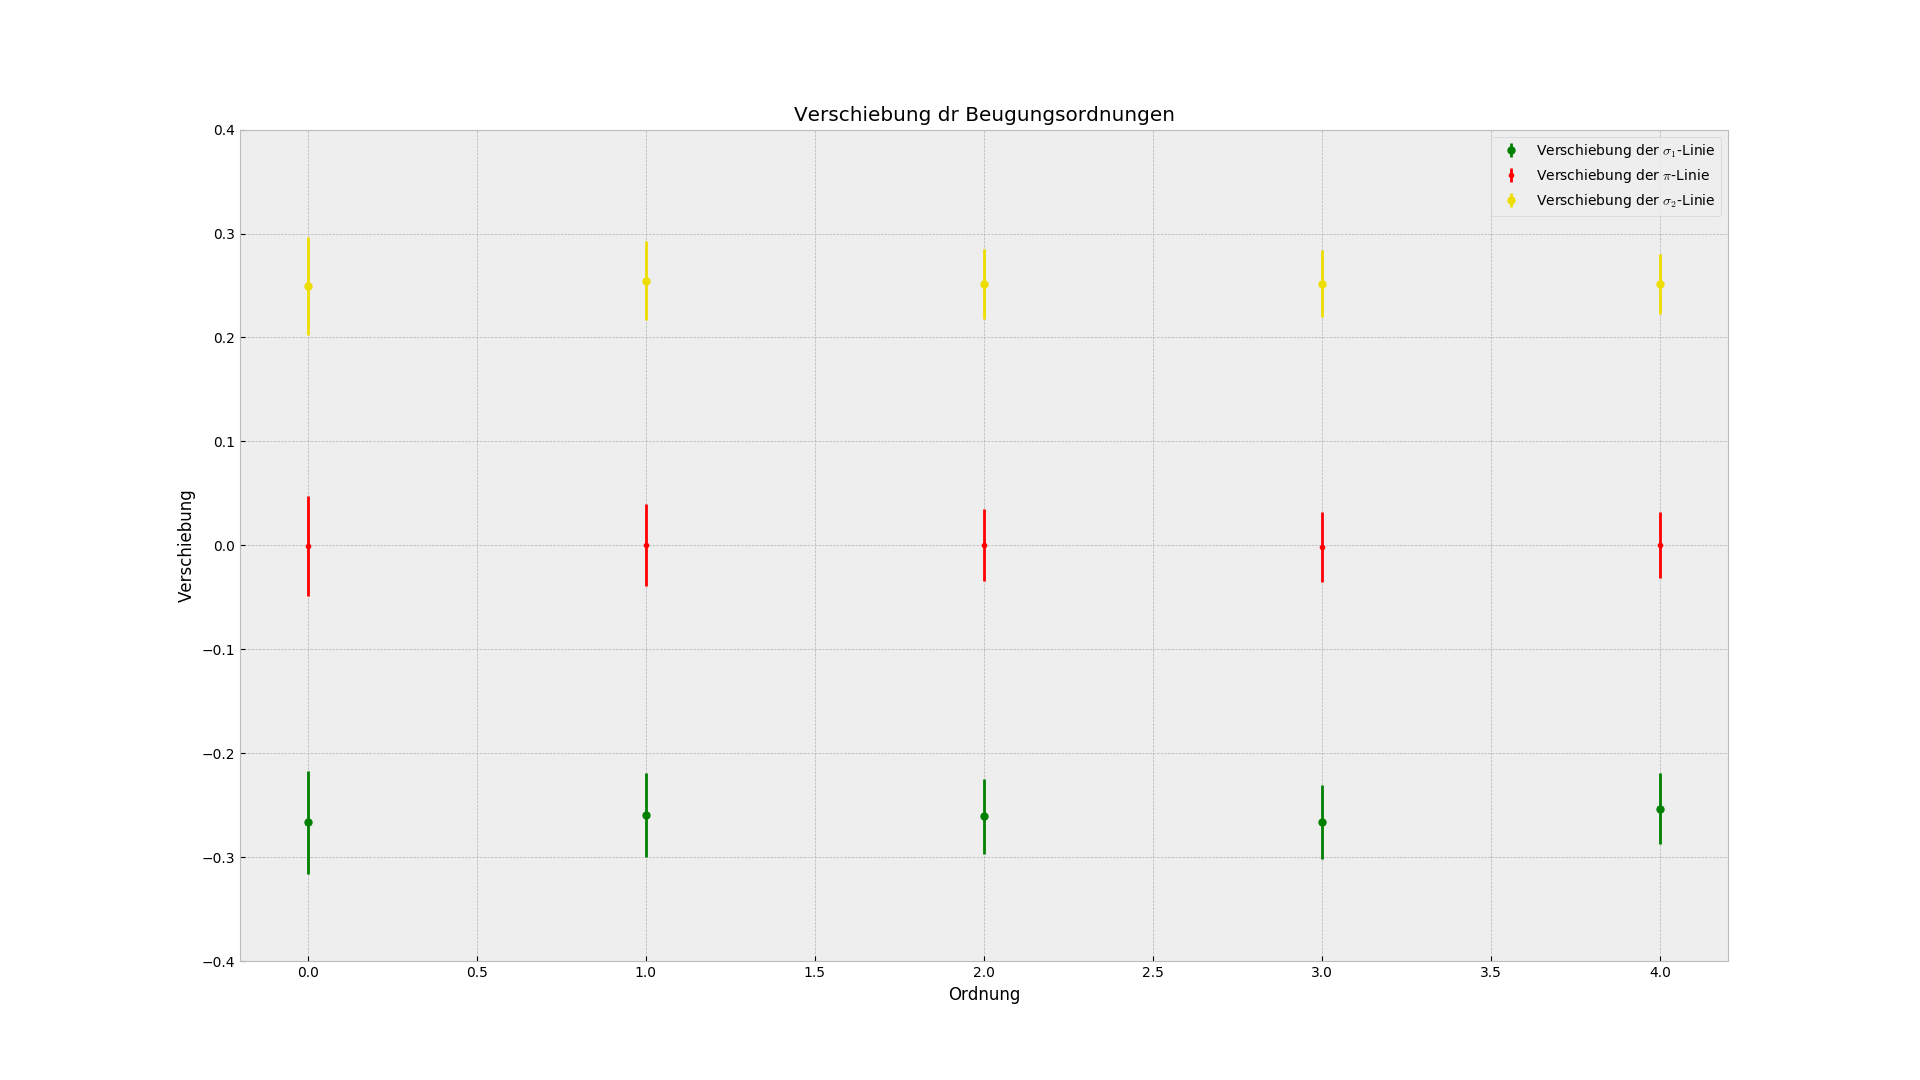
\includegraphics[width=.45\paperwidth]{Auswertung/scatterorder/diff_sco12A}
            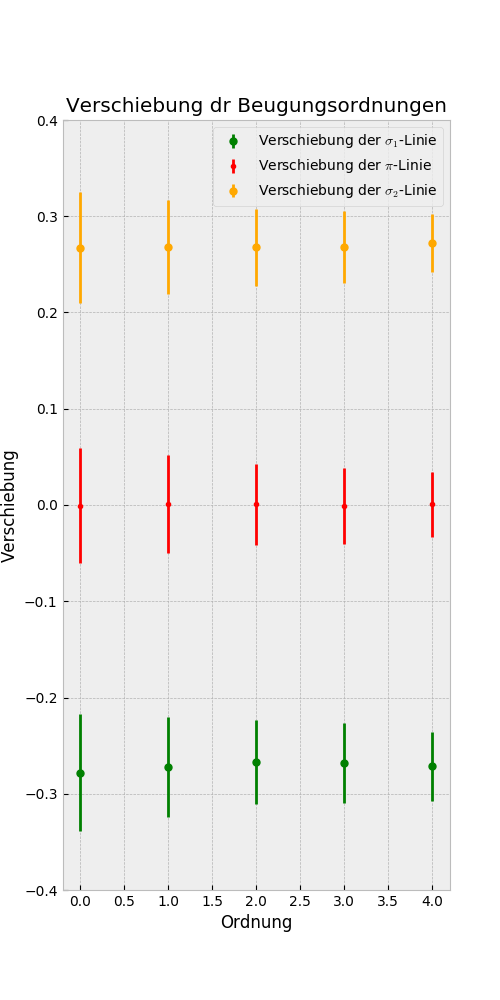
\includegraphics[width=.45\paperwidth]{Auswertung/scatterorder/diff_sco13A}
          \end{figure}
        \end{landscape}

      \subsubsection{Wellenlängenverschiebung}
        Um die Verschiebung der Wellenlänge zu erhalten nutzen wir die errechneten Werte in Bruchteilen der Beugungsordnung.
        \begin{align}
          \delta \lambda = \frac{\delta a}{\Delta a}\cdot \Delta \lambda \approx \delta k\cdot \Delta\lambda \label{fml::2}
        \end{align}
        Wobei die benutzte Näherung nur für kleine Verschiebungen gilt, in der der betrachtete Bereich der quadratischen Funktion als linear angesehen werden kann. Mithilfe von \hyperref[fml::1]{Gl. (\ref*{fml::1})}
        und \hyperref[fml::2]{Gl. (\ref*{fml::2})} kann jetzt die Wellenlängenverschiebung berechnet werden. Für die Wellenlänge $\lambda_{Cd}$ der roten Cadmium-Linie sowie deren Fehler verwenden wir den in Teil 2 ermittelten Wert \hyperref[val::lcd]{Gl. (\ref*{val::lcd})}:
        \begin{align}
          \lambda_{Cd} = \SI{643.927+-0.571}{\nano\metre}
        \end{align}
        ($n = \SI{1.4567}{}, d=\SI{4.04e-3}{m}$)

        Aus den Ergebnissen der untersuchten Ordnungen (\hyperref[plot::3.5]{Abb. \ref*{plot::3.5}}) lässt sich ein Mittelwert mit statistischem Fehler berechnen, um so jeweils einen Wert für die Wellenlängenverschiebung der beiden σ-Linien zu erhalten. Da das Experiment bei drei verschiedenen Magnetfeldern durchgeführt wurde, ergeben sich so sechs Werte, die nachfolgend in einer Tabelle zusammengefasst sind.
        \begin{table}[H]
          \centering
          \begin{tabular}{lll}
\toprule
I/A & $\delta\lambda_1/\si{pm}$ & $\delta\lambda_2/\si{pm}$ \\
\midrule
 10 &       $-11.394 \pm 0.140$ &        $10.788 \pm 0.294$ \\
 12 &       $-12.656 \pm 0.239$ &        $12.197 \pm 0.087$ \\
 13 &       $-13.153 \pm 0.187$ &        $13.019 \pm 0.093$ \\
\bottomrule
\end{tabular}

          \caption{Wellenlängenverschiebung für die drei beobachteten Stromstärken, sowie für beide $\sigma$-Linien}
          \label{tab::1}
        \end{table}

      \subsection{Bestimmung des Bohr'schen Magnetons}
        Das äußere Magnetfeld verursacht eine Verschiebung des Energieniveaus in Cadmium, diese Differenz lässt sich mit Hilfe der zuvor bestimmten Wellenlängenverschiebung der Spektrallinien berechnen:
        \begin{align}
          \Delta E         &= \frac{hc}\lambda-\frac{hc}{\lambda+\delta\lambda}\\
          \Delta(\Delta E) &= \frac{hc}{(\lambda+\delta\lambda)^2}\cdot\Delta(\delta\lambda)
        \end{align}
        Zwischen angelegtem Magnetfeld und der Energieverschiebung gilt \hyperref[fml::3]{Gl. (\ref*{fml::3})}

        Wir bestimmen das Magneton nun auf zwei unterschiedliche Arten:

        \subsubsection{Methode 1 - statistisches Mittel}
          Wir kennen jetzt die Werte des Magnetfeldes, sowie die entsprechende Energieverschiebung und können nun das Magneton berechnen:
          \begin{align}
            \mu_B=\left| \frac{\Delta E}{B} \right|
          \end{align}
          Wir erhalten erneut sechs Werte, sowie deren Fehler:
          \begin{table}[H]
            \centering
            \begin{tabular}{lll}
\toprule
I/A & $\mu_{B1}/(10^{-24}\si{\joule\per\tesla})$ & $\mu_{B2}/(10^{-24}\si{\joule\per\tesla})$ \\
\midrule
 10 &                         $10.446 \pm 0.461$ &                          $9.890 \pm 0.499$ \\
 12 &                         $10.090 \pm 0.452$ &                          $9.724 \pm 0.401$ \\
 13 &                          $9.845 \pm 0.418$ &                          $9.744 \pm 0.396$ \\
\bottomrule
\end{tabular}

            \caption{Bohr'sches Magneton, nach Methode 1, für beide $\sigma$-Linien}
            \label{tab::2}
          \end{table}~\\
          Der gesamte Mittelwert aus diesen Daten ist dann:

          \begin{align}
            \mu_B         &= \magnetonOne\\
            \mu_{B, theo} &= \magnetonTheo %TODO insert source
          \end{align}
          Der hier ermittelte Wert und der gegebene Theoriewert stimmen dabei innerhalb von \SI{1.6}{\sigma} überein.

        \subsubsection{Methode 2 - linearer Fit}
        Der lineare Zusammenhang, zwischen Magnetfeld und Energieverschiebung, lässt auch eine graphische Bestimmung des Bohr'schen Magnetons zu. Hier wird die Energieverschiebung gegen das Magnetfeld aufgetragen und linear gefittet. Die Steigung dieses Fits entspricht dem Wert für das Bohr'sche Magneton. Der Mittelwert beider Werte gibt das Endergebnis an.

        \begin{align}
          \mu_B = \magnetonTwo
        \end{align}
        Allerdings liegt hier die Abweichung zum Literaturwert bei \SI{4.2}{\sigma}, und ist somit signifikant.
        \begin{figure}[H]
          \centering
          \hspace*{-1.5cm}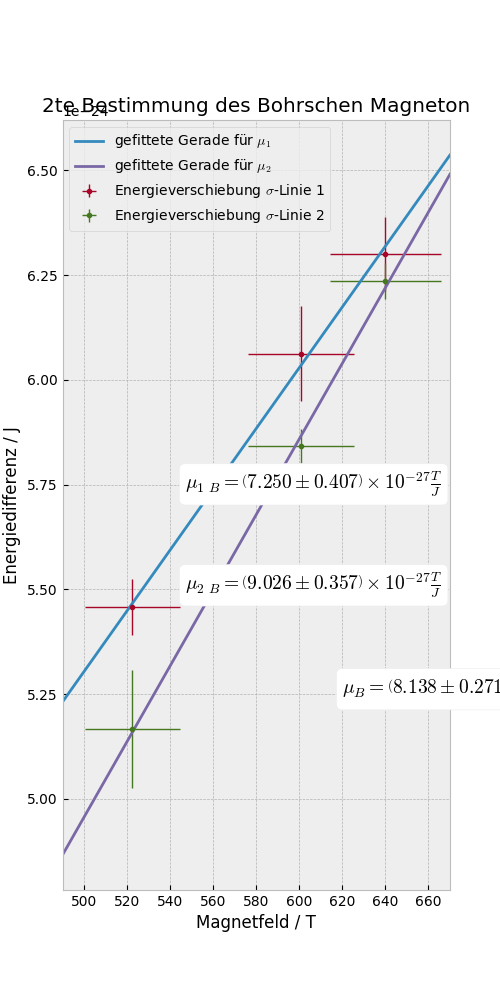
\includegraphics[width=1.2\textwidth]{Auswertung/mu_B2}
          \caption{Graphische Bestimmung des Bohr'schen Magneton}
          \label{plot::4}
        \end{figure}
